\documentclass{article}
\usepackage{graphicx} % Required for inserting images
\usepackage{authblk} % For author affiliations
\usepackage{hyperref} % For hyperlinks
\usepackage[margin=1in]{geometry} % Standard margins
\usepackage{natbib} % For bibliography management
\usepackage{enumitem} % For customising lists
\usepackage{color}
\usepackage{amsmath}
\usepackage{float}
\usepackage{booktabs}
\newlist{tree}{itemize}{10}
\setlist[tree]{label=-}
\setlistdepth{10} 


\title{Integrating Multiple Data Sources in Infectious Disease Modelling: Best Practices and Implementation}

\author[1]{Sam Abbott}
\author[2]{Xiahui Li}
\author[3]{Punya Alahakoon}
\author[4]{Dhorasso Junior Temfack Nguefack}
\author[5]{Johannes Bracher}
\author[6]{Felix Günther}
\author[7]{@working-group-members}
\author[8]{@workshop-participants}
\author[9]{Mircea T. Sofonea}
\author[10]{Michael Plank}
\author[11]{Anne Presanis\thanks{Joint last authors}}
\author[12]{Anne Cori$^*$}

\affil[1]{London School of Hygiene \& Tropical Medicine}
\affil[2]{University of St Andrews}
\affil[3]{University of Oxford}
\affil[4]{Trinity College Dublin}
\affil[5]{Karlsruhe Institute of Technology}
\affil[6]{Robert Koch Institute}
\affil[7]{@working-group-affiliations}
\affil[8]{@workshop-participant-affiliations}
\affil[9]{University of Montpellier, France}
\affil[10]{University of Canterbury, New Zealand}
\affil[11]{MRC Biostatistics Unit, University of Cambridge}
\affil[12]{Imperial College London}

% Note: Author order is provisional and subject to change

\date{\today}

\begin{document}

\maketitle

\begin{abstract}
The increase in available data sources during recent infectious disease outbreaks has created both opportunities and challenges for modellers seeking to integrate diverse data streams.
Whilst rigorous Bayesian workflow practices have been established in other fields, the infectious disease modelling community has been slow to adopt these approaches, despite working in rapidly evolving settings where novel data sources emerge and surveillance systems adapt in real-time.
This paper provides a methodological framework for integrating multiple data sources in infectious disease modelling, with transmission intensity estimation as a key exemplar.
We characterise data source properties through a structured survey of workshop participants and present an iterative workflow that extends established Bayesian model development approaches to the infectious disease domain.
Our workflow progresses from research question definition through development of directed acyclic graph (DAG) representations of process and observation, to integration method selection, with explicit consideration of data conflicts and uncertainty quantification.
We compare integration approaches, from full joint modelling to modular ensemble methods, and demonstrate through schematic case studies how practitioners can navigate real-world tradeoffs between model complexity, computational feasibility, and inferential goals.
The case studies show how different data types, including individual-level observations, provide complementary information for estimating parameters such as time-varying reproduction numbers and overdispersion of transmission dynamics.
Throughout, we advocate Bayesian thinking for principled model development, regardless of the ultimate fitting approach.
Our framework emphasises parsimony, interpretability, and data conflict assessment, addressing a critical gap by providing practical guidance supported by schematic worked examples.
\end{abstract}

\section{Introduction}
% Lead: Sam Abbott

% Paragraph 1: Motivation and Context
Infectious disease modelling increasingly relies on integrating multiple data sources to improve parameter estimation, reduce uncertainty, and provide more robust evidence for public health decision making [@placeholder].
Recent outbreaks including COVID-19, mpox, and Ebola have highlighted both the potential value and practical challenges of combining diverse data streams such as case reports, deaths, hospitalisations, genomic sequences, wastewater surveillance, and serological surveys [@placeholder].
These outbreak settings create unique pressures where novel data streams emerge rapidly, surveillance systems evolve to meet changing needs, and models must be developed under severe time constraints with limited understanding of new data sources [@placeholder].
Single data sources often provide limited or biased information about key epidemiological parameters, whilst multiple sources can offer complementary perspectives that improve model accuracy and reliability [@placeholder].
However, practitioners face complex methodological choices about how to combine these data streams effectively.

% Paragraph 2: Current Approaches
Current approaches to multi-source integration broadly fall into two categories: pipeline methods that fit separate models to individual data sources before combining estimates, and joint modelling approaches that simultaneously fit all data sources within a unified statistical framework \citep{deangelis2018analysing, russell2024combined}.
Pipeline approaches offer computational efficiency and modular development, but may propagate errors and fail to capture dependencies between data sources [@placeholder].
Joint modelling can provide more principled uncertainty quantification and better parameter identifiability, but often requires substantial computational resources and model complexity \citep{russell2024combined, lison2024generative}.
Recent empirical evidence demonstrates that joint approaches consistently outperform stepwise methods by avoiding error propagation and improving parameter identifiability \citep{lison2024generative}.
Beyond these choices, practitioners face numerous challenges including: detecting and resolving conflicts between data sources; combining data sources with different spatial or temporal resolutions; validating models when different data streams suggest different dynamics; and navigating branching decision paths where integration choices impose model structure constraints [@placeholder].
Fitting challenges, such as computational intractability, parameter non-identifiability, and the need to approximate ideal model structures for practical inference, further complicate implementation [@placeholder].
These integration and fitting considerations can impact model design, yet their implications are rarely made explicit in published analyses [@placeholder].
The infectious disease modelling community has not widely adopted rigorous Bayesian workflow practices that emphasise iterative model development, systematic model criticism, and principled uncertainty quantification \citep{gelman2020bayesian, nicholson2022interoperability}.
Existing guidance for practitioners is fragmented across methodological literature, with limited practical frameworks for navigating these interconnected choices systematically [@placeholder].

% Paragraph 3: Paper Scope and Contribution
This paper provides a framework for integrating multiple data sources in infectious disease modelling, with practical implementation as the primary focus.
We use the estimation of transmission intensity —specifically time-varying reproduction numbers and overdispersion parameters—as a case study to demonstrate broader principles applicable across infectious disease modelling contexts.
By focusing on this fundamental and widely-used estimation task, we provide practitioners with a concrete foundation for adopting rigorous workflow practices that can then be extended to more complex modelling challenges.
Our approach, building on established Bayesian workflows [@placeholder], encourages iterative model building with principled uncertainty quantification, allowing practitioners to systematically assess the value of additional data sources while maintaining interpretability and computational tractability.
We advocate for Bayesian thinking throughout the model development process—including careful prior specification, model criticism, and posterior predictive checks—regardless of whether the final implementation uses Bayesian or frequentist fitting methods.
The framework addresses critical gaps in existing literature by providing domain-specific guidance and signposting to more generic resources for integration choices, validation strategies, and conflict resolution between data sources.

% Paragraph 4: Paper Structure
We first review data source characteristics and present a structured iterative workflow for model development that progresses from research question definition through development of directed acyclic graphs (DAGs) representing process and observation, to integration method selection.
We then compare integration approaches from full joint modelling to modular ensemble methods.
Three worked case studies demonstrate progressive complexity: single-source baselines, two-source integration, and multi-stream applications incorporating individual-level data.
Each case study follows our iterative workflow, demonstrating how DAG-based model development guides data integration decisions and integration and fitting requirements can feedback into model design.

\section{Data Sources and Characteristics} \label{sec:datareview}
% Lead: Punya Alahakoon

\paragraph{}In this study, we consider incorporating diverse data sources, including time-series case and hospitalisation data, wastewater data, and XXX. To systematically evaluate these data, we identified six key components that characterise their structure and utility: metadata, scope,  resolution, data quality, data utility, and practical considerations. For each component, we defined a set of attributes based on [XXX and YYY ??] that can serve as a set of guidelines for assessing strengths and limitations of a given data stream. 

\paragraph{}\textit{Metadata} encapsulates the foundational information about each data stream. This includes the classification of data, descriptive attributes, the study design underpinning its collection, and the primary objectives for which data were originally gathered. 

\paragraph{}The \textit{scope} of a data source refers to the representative breadth and epidemiological relevance of a data source [CITE]. This may include characteristics of the population captured by the data, and the degree to which it captures the source population. The scope further encompasses the intended target population, the potential for stratification by demographic, clinical, or other attributes, and the mode of data collection---whether it is routine, event-triggered or a one-off. 

\paragraph{}\textit{Resolution} may describe the granularity and the level of details captured by a data source. This includes whether the data are collected at an individual or aggregated level, as well as the temporal and spatial precision of the measurement. High-resolution data may offer fine-grained time stamps (e.g., daily, hourly) and details geographic identifiers (e.g., international, national), which are essential for modelling transmission dynamics and identifying localised outbreaks. 

\paragraph{} \textit{Data quality} component encompasses the reliability, accuracy and completeness of the measurements within a data stream. Key aspects of this component may include quality of the case definitions, diagnostic test performance (test sensitivity and specificity), and the presence of reporting delays. It may also involve identifying and quantifying potential sources of biases such as missing data, truncation and censoring. Furthermore, these biases may be time-varying and directional, which is also a characteristic of this component. 

\paragraph{}\textit{Data utility} refers to the practical applicability of a data source in informing epidemiological metrics and supporting public-health decision making. This component identifies which transmission-related quantities---such as incidence, prevalence, and the basic reproduction number---can be inferred from the data, and if so, if they can be directly or indirectly calculated. Data utility can also characterise whether insights derived from the target population can be generalised to broader populations, and evaluate the extent to which the data support these generalisations.  

\paragraph{} \textit{Practical considerations} address the feasibility of using a data stream in modelling and surveillance contexts. This may include factors such as scalability, sustainability, and cost-effectiveness of data collection. It also considers the ease of integration with other data sources, including data format compatibility and linkage potential. Additional considerations may include the generalisability of the data stream to other pathogens or settings. 

\paragraph{}Figure \ref{data_characteristics} illustrates the proposed six core components used to characterise data streams, along with representative attributes that can be used to assess their strengths and limitations. We note that the relevance and performance of these characteristics may vary across data sources and are inherently dependent on the specific objectives for which data are being used, and which multiple sources of data are intended to be integrated. These considerations are discussed in more detail in Section XXX (case studies), where we examine specific data sources in applied contexts.  

\begin{figure}[H] 
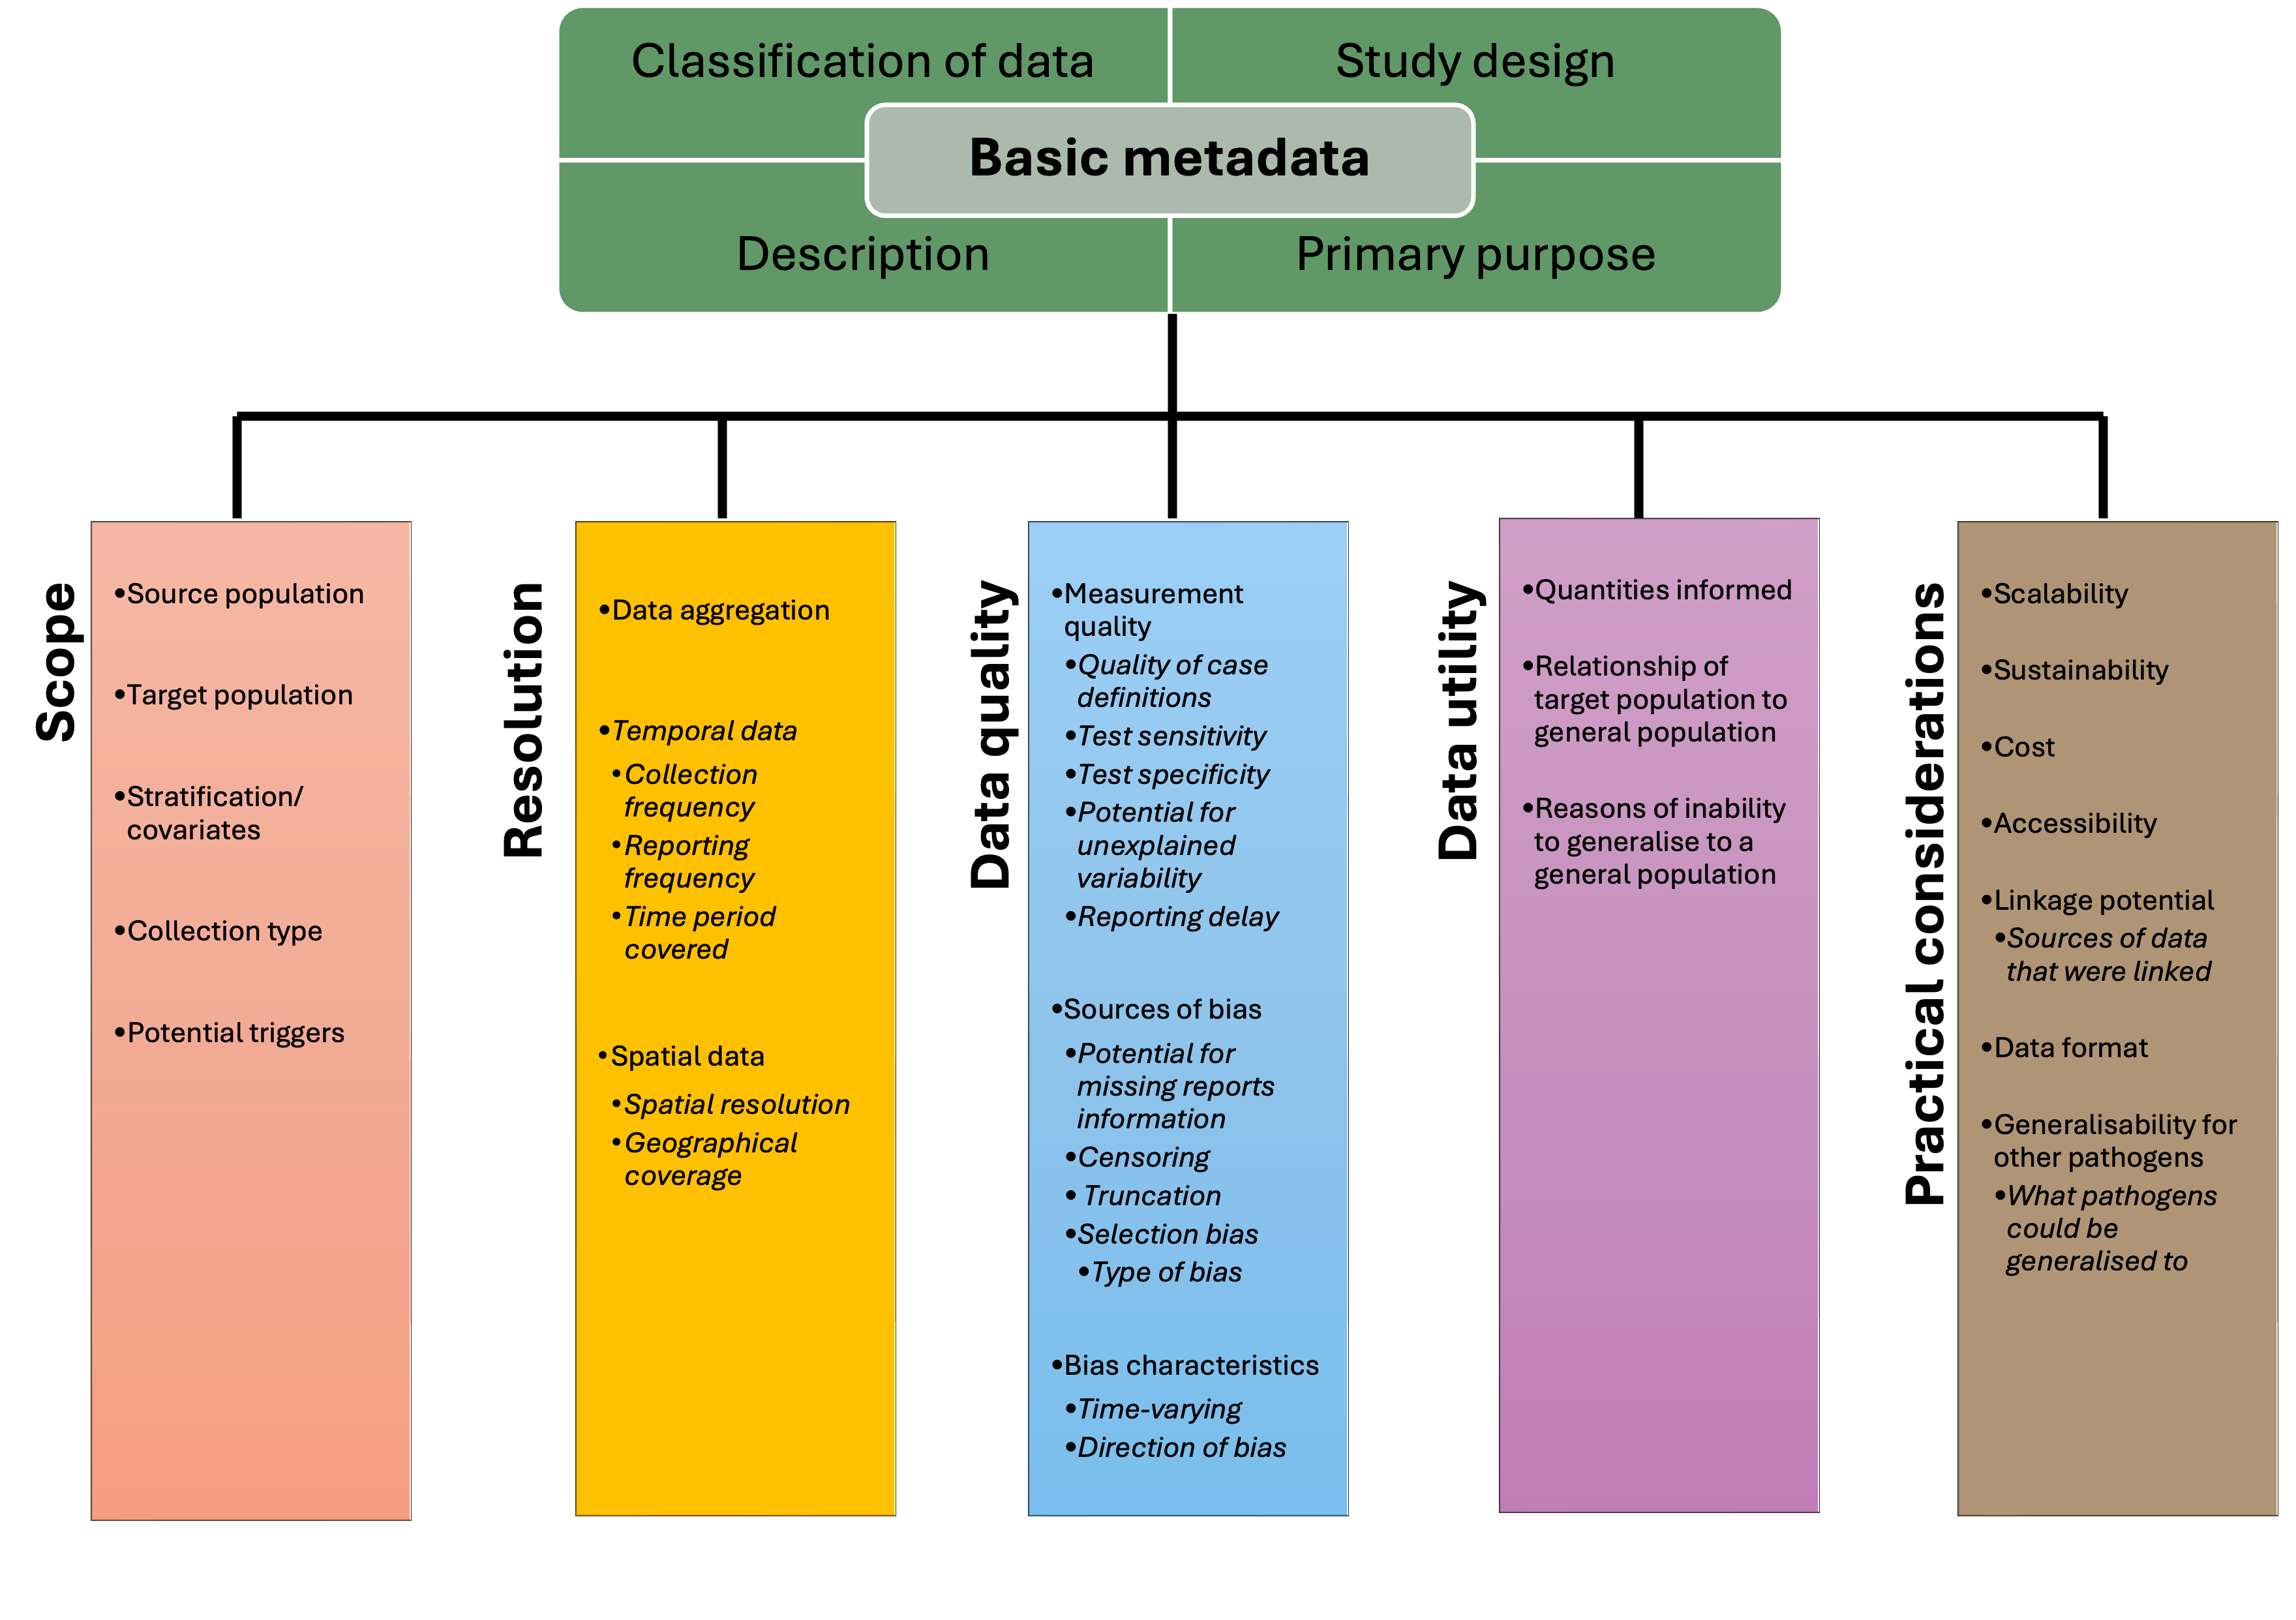
\includegraphics[width=1\linewidth]{figures/data_characteristics.png}
\centering
\caption{The proposed framework for characterising a data stream used in infectious disease surveillance and modelling. The six core components---metadata, scope, resolution, data quality, data utility and practical considerations---are illustrated alongside representative attributes that can be used to assess the strengths and limitations of each data source. }
\label{data_characteristics}
\end{figure}


%Participants evaluated candidate datasets across six main categories: basic metadata, scope, resolution, data quality, data utility, and practical considerations.
%For each subcategory, experts assigned values between 0 and 5, selected appropriate categories, or provided free text responses.
%We harmonised and ensembled these expert assessments to create overview tables and data analysis.

% TODO: Present survey results and expert consensus
% TODO: Create comprehensive table of data characteristics  
% TODO: Discuss taxonomy of data sources in infectious disease surveillance
% TODO: Analyse information content and complementarity
% TODO: Address preprocessing and standardisation requirements

\section{Workflow}
% Lead: Sam Abbott

\subsection{Overview}

We recommend following a structured, iterative workflow for multi-data source modelling (Figure~\ref{fig:workflow}), building on established Bayesian workflow principles [@gelman2020bayesian].


\begin{figure}[htbp]
    \centering
    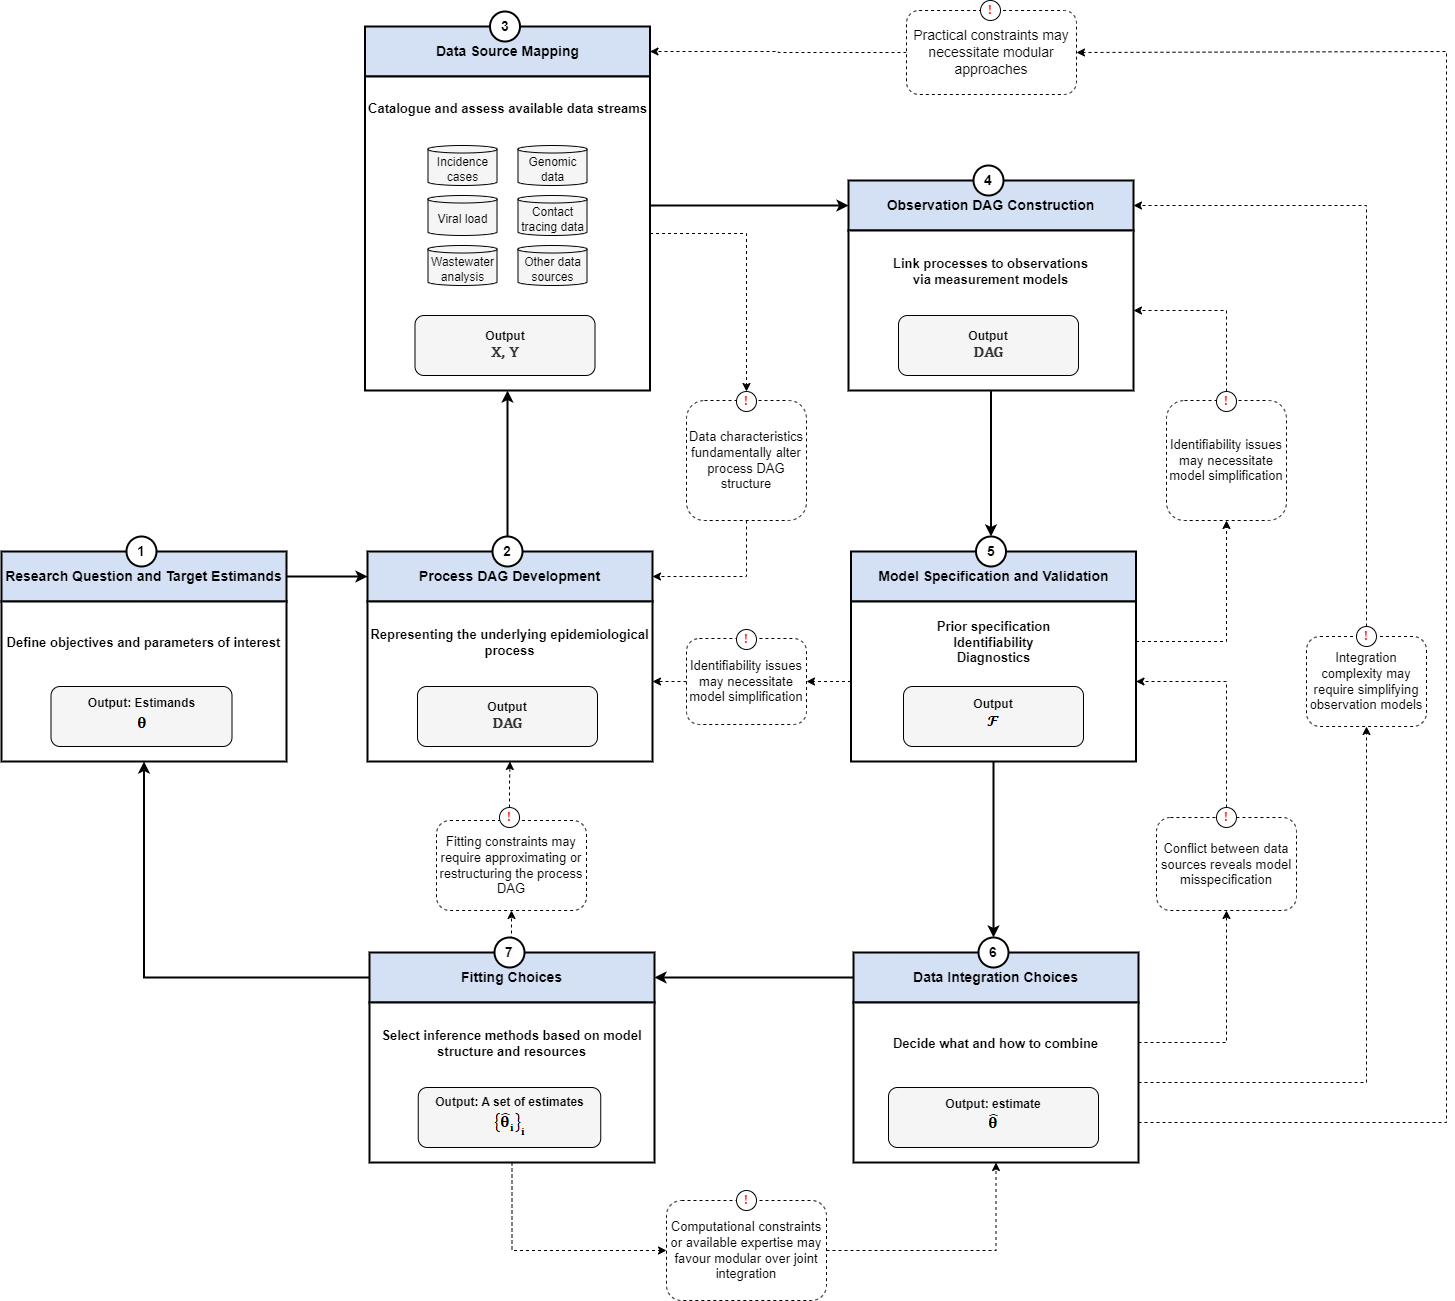
\includegraphics[width=\textwidth]{figures/visualization of core steps.drawio.png}
    \caption{Recommended workflow for integrating multiple data sources in infectious disease modelling. Begin by defining research questions and target estimands, proceed through iterative development of process and observation DAGs, and follow critical decisions about data integration and inference methods. Note the feedback loops where downstream choices constrain or inform upstream model development.}
    \label{fig:workflow}
\end{figure}

Our suggested workflow extends established Bayesian workflow principles—with their emphasis on iterative model building, prior predictive checks, computational diagnostics, and posterior predictive assessment—to the specific challenges of multi-source infectious disease modelling.
A key distinguishing feature is the explicit separation of epidemiological process DAGs from observation DAGs, recognising that whilst these components interact through feedback mechanisms, they draw from different domains: epidemiological processes are informed by infectious disease theory whilst observation models are motivated by data source characteristics and collection mechanisms.
Start with a clear research question, such as estimating transmission intensity—, and use systematic model development through directed acyclic graphs (DAGs) with iterative refinement.
We advocate this approach because it makes modelling choices transparent, assumptions explicit, and provides principled tools for assessing model adequacy regardless of whether final inference is Bayesian or frequentist.

We recommend beginning with \textbf{decision making}: clearly define your research question and target estimands (e.g., time-varying reproduction number, overdispersion parameters).
Next, develop a \textbf{process DAG} representing the underlying epidemiological process, iterating on this representation as understanding develops.
Map available \textbf{data sources} to your process model, such as incidence time series, genomic data, contact tracing, viral load measurements, and serological surveys based on those identified in the previous section.
For each data source, develop an \textbf{observation DAG} linking the underlying process to observed data through measurement models and reporting mechanisms.
Different data sources may also impact your \textbf{process DAG} assumptions, such as if you can collapse your representation of the process from individual-level to population-level so there needs to be a model feedback loop.

Once you have developed your process and observation DAGs, proceed to \textbf{model specification and validation}, including prior specification, parameter identifiability assessment, and diagnostic approaches.
You then face the key decisions: \textbf{``What to combine?''} and \textbf{``How to combine?''}.

If combining multiple sources is not beneficial or feasible, you can proceed to single-source modelling and combination of estimates.
If integration is warranted, select among data integration methods including full joint modelling, modular techniques, Markov melding, or approximate weighting approaches. Again, fitting or computational constraints (e.g., NUTS inability to handle discrete latents) may require revising the process DAG or data integration choices. 
Finally, fit your model and evaluate its performance through posterior predictive validation and sensitivity analysis.

The workflow can be summarised as follows:

\textbf{Core Workflow Components:}
\begin{enumerate}
    \item \textbf{Research Question and Target Estimands} - Define your objectives and parameters of interest
    \item \textbf{Process DAG Development} - Represent the underlying epidemiological process
    \item \textbf{Data Source Mapping} - Catalogue and assess available data streams
    \item \textbf{Observation DAG Construction} - Link processes to observations via measurement models
    \item \textbf{Model Specification and Validation} - Prior specification, identifiability, diagnostics
    \item \textbf{Data Integration Choices} - Decide what and how to combine
    \item \textbf{Fitting Choices} - Select inference methods based on model structure and resources
\end{enumerate}

\textbf{Key Feedback Loops:}
\begin{itemize}
    \item Components 3→2: Data characteristics (e.g., individual-level vs population-level) fundamentally alter process DAG structure
    \item Components 5→2,4: Identifiability issues may necessitate model simplification
    \item Components 6→3: Practical constraints (e.g., different teams using incompatible programming languages) may necessitate modular approaches
    \item Components 6→4: Integration complexity may require simplifying observation models
    \item Components 6→5: Conflict between data sources reveals model misspecification
    \item Components 7→2: Fitting constraints (e.g., NUTS inability to handle discrete latents) may require approximating or restructuring the process DAG
    \item Components 7→6: Computational constraints or available expertise may favour modular over joint integration
\end{itemize}

The multiple feedback loops mean that model development is rarely a single forward pass through the workflow. For example, if you initially design a joint model but find it computationally intractable with available methods, you might iterate back to choose a modular integration approach, which in turn might influence how you structure your observation DAGs.
Similarly, if MCMC convergence fails due to discrete latent parameters, you might need to marginalise them out or adopt a different process representation.

In the following sections, we will discuss each of these steps in more detail.

\subsection{Research Question and Target Estimands}
% TODO: Defining clear research objectives
% TODO: Specifying target parameters and estimands
% TODO: Connecting questions to policy needs - actually I think it's maybe connecting epidemiological parameters with policy questions
% TODO: Setting scope and boundaries

\begin{itemize}
\item \textbf{Multi-source research questions:} Identify when multiple data streams are necessary for robust inference. For example, reproduction number estimation benefits from combining case reports with hospitalisation data to account for different population subgroups and reporting biases \citep{sherratt2021exploring}.

\item \textbf{Causal estimand clarification:} Use DAG principles to distinguish between total effects and pathway-specific effects when integrating data sources. Testing rates may mediate relationships between policy interventions and observed case counts, requiring careful estimand specification \citep{digitale2022tutorial}.

\item \textbf{Estimand specification:} Map research questions to specific parameters requiring multi-source data. Variant-specific transmission advantages require integration of genomic surveillance with epidemiological time series \citep{abbott2021estimating}.

\item \textbf{Source complementarity:} Identify how different data sources provide complementary information. Early warning signals from wastewater surveillance can be confirmed through clinical surveillance systems \citep{ro2025estimating}.
\end{itemize}

\subsection{Process DAG Development}
% TODO: Representing epidemiological processes
% TODO: Causal relationships and assumptions
% TODO: Iterative refinement based on understanding
% TODO: Incorporating biological mechanisms

\begin{itemize}
\item \textbf{State-space framework:} Develop directed acyclic graphs separating epidemic processes from observation mechanisms, following the Bayesian evidence synthesis framework for epidemic data integration \citep{deangelis2018analysing}.

\item \textbf{Causal identification:} Use DAG principles to identify confounders, mediators, and colliders when integrating multiple data sources, ensuring minimal adjustment sets for unbiased estimation \citep{digitale2022tutorial}.

\item \textbf{Hierarchical structure:} Account for population heterogeneity and demographic stratification when multiple data sources capture different population subgroups \citep{russell2024combined}.

\item \textbf{Selection bias prevention:} Map data collection processes to identify potential collider structures, particularly when surveillance systems have differential participation patterns \citep{digitale2022tutorial}.

\item \textbf{Causal relationships:} Explicitly represent relationships between transmission processes, interventions, and observed data streams to enable modular model development \citep{nicholson2022interoperability}.
\end{itemize}

\subsection{Data Source Mapping}
% TODO: Cataloguing available data streams
% TODO: Assessing data characteristics and biases
% TODO: Linking data to process components
% TODO: Evaluating complementarity and redundancy

\subsection{Iterate on the Process DAG}

%TODO: based on available data sources and the original process DAG may need to iterate
%TODO: An example is the need for individual level modelling for certain data sources which might impact the construction of the process DAG.

\subsection{Observation DAG Construction}
% TODO: Measurement models and reporting processes
% TODO: Delays and missing data mechanisms
% TODO: Linking latent processes to observations
% TODO: Accounting for data collection protocols

\subsection{Model Specification and Validation}\label{sec:spec-validate}
% TODO: Bayesian workflow principles
% TODO: Prior specification and prior predictive checks
% TODO: Parameter identifiability assessment
% TODO: Model criticism and diagnostic approaches
% TODO: Posterior predictive validation
% TODO: Cross-validation strategies
% TODO: Sensitivity analysis frameworks

\begin{itemize}
\item \textbf{Multi-source diagnostics:} Implement cross-stream validation where each data source validates others, extending standard convergence diagnostics \citep{sherratt2021exploring}.

\item \textbf{DAG-based validation:} Test causal assumptions underlying multi-source integration using sensitivity analyses and, where possible, natural experiments to validate DAG structures \citep{digitale2022tutorial}.

\item \textbf{Bias detection:} Monitor for selection bias patterns across different surveillance systems, particularly when participation differs systematically between data sources \citep{digitale2022tutorial}.

\item \textbf{Decision-focused evaluation:} Assess model performance based on decision utility rather than purely statistical metrics, particularly important for policy-relevant multi-source applications \citep{marshall2024when}.

\item \textbf{Computational validation:} Apply systematic diagnostic frameworks to complex multi-source models, ensuring proper uncertainty propagation across data streams \citep{gelman2020bayesian}.
\end{itemize}

\subsection{Data Integration Choices}
% Lead: Anne Presanis

%Consideration: How do we clearly split here between combined and individual approaches? What does that structure look like? How do we connect this question to fitting choices which in practice are important?
%Consideration: What parts of this (sub models etc etc are part of specification and validation. How does that interaction work?
%Consideration: There might be an ideal DAG structure but in practice need to approximate for fitting. I.E want to use NUTs so can't have latent discrete parameters etc...

\subsubsection{Decision Framework}
% When to integrate vs when to keep separate
% Assessing complementarity and redundancy
% Computational vs inferential trade-offs

In principle, integrating multiple data should enhance the identifiability and precision of parameter estimates (REFS). Even when data streams are redundant (informing the same quantity), their combination can improve precision, consistent with meta-analytic principles (REF). 

In practice, however, data integration may pose challenges. These include inconsistencies due to unaccounted biases (REFS); computational complexity (REFS); and real-time pressures during an outbreak emergency (REF).

Evaluating the strengths and limitations of different data sources, as described in Section \ref{sec:datareview}, can and should be done during inter-epidemic periods. This evaluation, alongside with the workflow of specifying process and observation DAGs (Section ??), helps assess whether estimands of interest are identifiable from the available data. Value-of-information methods(REFs) can further guide whether new or additional, data would meaningfully improve precision. However, for complex models especially, identifiability may only become evident after fitting an initial version.

Decisions about data integration are inherently context-dependent, but can be guided by the decision tree in Figure \ref{fig:integration}. When combining independant model outputs from different groups, the choice of ensembling or meta-analytic approach should align with the research objective (e.g. estimation or prediction), and influence how estimates or predictions are weighted (e.g. by precision or prediction accuracy). In contrast, when integrating sub-models, the approach will depend on whether existing sub-models have already been fitted, or if the models are being developed de novo.

\subsubsection{Integration Methods}
% Modular approaches and staged fitting
% Markov melding
A modular model building approach (REFs) is generally preferable, buided by the principle of parsimony (``Occam's razor'', REF). 
Starting with simple sub-models makes it easier to diagnose issues such as poor fit, model misspecification or convergence issues. Complexity can then be added incrementally, only as far as needed. Sequentially combining sub-models also dacilitates the detection of inconsistencies or conflicts between them (REFs). 

Modular approaches offer computational advantages. Techniques like Markov melding (REF) allow posterior samples from one sub-model to serve as a proposal distributions for the next, avoiding the need to refit a full joint model. This sequential strategy, using the posterior from one sub-model as the prior for another, have a long history (REF?). 
While the theory and some applications of Markov melding are well-established (REFs), practical implementation remains challenging. Limitations include the availability of user-friendly Bayesian software 
and methods for assessing sub-model compatibility (REF). As a result, approximate methods are often used. A common approach 
is to combine a Stage 1 estimate with a Stage 2 model by assuming the Stage 1 point estimate is a realisation (on an appropriate scale) of a Normal distribution with fixed variance given by the squared Stage 1 standard error or posterior standard deviation (REFs). This mirrorsstandard meta-analysis techniques (REF); and has been shown to be an approximation to Markov melding with ``product of experts'' pooling, considering a Normal approximation for the Stage 1 sub-model (REF).

% Cut distribution and generalised evidence synthesis
Modular approaches also support selective trust in sub-models. ``Cutting'' feedback - i.e. preventing less reliable sub-models from influencing more trusted ones while allowing the reverse — enables nuanced evidence synthesis(REFs).

% TODO: Full joint modelling
% suggested text from copilot in case useful:
% Full joint modelling offers a coherent framework for integrating multiple data sources and processes simultaneously. By specifying a single joint likelihood and prior structure, this approach can capture dependencies and interactions across sub-models more naturally than modular alternatives. It is particularly valuable when feedback between components is essential or when sub-models are tightly coupled.
% However, joint models can be computationally intensive and challenging to fit, especially in high-dimensional or real-time settings. They also require careful specification to avoid identifiability issues and to ensure that all components are appropriately informed by the data. Despite these challenges, joint modelling remains the gold standard when feasible, offering the most principled basis for inference.

% TODO: Ensemble and weighting methods
% suggested text from copilot in case useful:
% When multiple models or estimates are available—whether from different research groups or alternative specifications—ensemble methods provide a flexible way to combine them. The choice of ensemble strategy should reflect the research objective. For prediction, weighting by out-of-sample accuracy may be appropriate; for estimation, weights might reflect precision or model credibility.
%Common approaches include Bayesian model averaging, stacking, and meta-analytic pooling. These methods can accommodate model uncertainty and allow for robustness across competing hypotheses. In practice, ensemble weights may be fixed, data-driven, or informed by expert judgment, depending on the context and available information.

\subsubsection{Practical Constraints}
% Different teams with different expertise/languages
% Software compatibility issues
% Computational resource limitations
% Time constraints in outbreak settings

% Copilot suggestion in case useful to flesh out the above:
% Despite the theoretical advantages of data integration and modular modelling, several practical constraints often limit their implementation in real-world settings:
%Diverse Teams and Disciplinary Silos: Collaborative modelling efforts frequently involve teams with varied disciplinary backgrounds, methodological preferences, and even programming languages. This diversity, while enriching, can complicate communication, model interoperability, and consensus on modelling frameworks.
%Software Compatibility: Differences in software ecosystems—such as R, Python, Stan, or proprietary tools—can hinder seamless integration of sub-models or data pipelines. Even when using the same language, variations in package versions or coding conventions can introduce friction.
%Computational Resources: High-dimensional models or those requiring extensive simulation (e.g., via MCMC) can be computationally demanding. Limited access to high-performance computing infrastructure may constrain the complexity or scale of models that can be feasibly implemented, particularly in low-resource settings.
%Time Constraints in Outbreak Settings: During public health emergencies, the need for rapid decision-making often precludes the development of fully integrated or optimised models. In such contexts, simpler or pre-existing models may be prioritised over more comprehensive but time-intensive approaches.
%These constraints highlight the importance of planning and infrastructure development during inter-epidemic periods, including the creation of interoperable modelling frameworks, shared codebases, and cross-disciplinary training.

\subsubsection{Conflict Detection and Resolution}
% Prior-data conflict
% Data-data conflict
% Model criticism in multi-source settings
% Sensitivity analysis approaches

% Copilot suggestion to flesh out the above in case useful:
%In multi-source modelling, detecting and resolving conflicts is essential to ensure coherent inference and robust decision-making. Conflicts can arise at various levels:
%Prior–Data Conflict: When prior beliefs are strongly contradicted by observed data, it may indicate misspecification or overly informative priors. Diagnostic tools such as prior predictive checks and posterior–prior overlap metrics can help identify such conflicts early in the modelling process.
%Data–Data Conflict: Different data sources may provide inconsistent evidence about the same underlying process, due to biases, measurement error, or contextual differences. Identifying these conflicts requires careful comparison of marginal likelihoods, posterior distributions, and model fit across data streams.
%Model Criticism in Multi-Source Settings: Traditional model criticism techniques—such as posterior predictive checks, residual analysis, and information criteria—must be adapted to account for the complexity introduced by multiple data sources. Modular approaches can help isolate problematic components, while joint models may require more sophisticated diagnostics.
%Sensitivity Analysis: Sensitivity analysis plays a key role in conflict resolution. Varying priors, data inclusion, or model structure can reveal the robustness of conclusions and help identify influential assumptions. In modular settings, sensitivity analysis can be performed component-wise, while in joint models, global sensitivity approaches may be more appropriate.
%Ultimately, conflict detection should be an iterative process, integrated into model development and refinement. Transparent reporting of conflicts and their resolution enhances the credibility and interpretability of modelling outputs, particularly in high-stakes settings such as outbreak response.


Attempt at tree of choices:
\begin{tree}
    \item Are you combining alternative/competing models from different groups?
    \begin{tree}
        \item Yes
        \begin{tree}
            \item How are the results from each available?
            \begin{tree}
                \item As point estimate and confidence/credible interval
                \begin{tree}
                    \item Do you trust the alternatives equally?
                    \begin{tree}
                        \item Yes $\Rightarrow$ standard meta-analysis
                        \item No
                        \begin{tree}
                            \item $\Rightarrow$ weighted meta-analysis, weighted by precision
                            \item $\Rightarrow$ or weighted by other criteria, e.g. prediction accuracy (ensembling)
                        \end{tree}
                    \end{tree}
                \end{tree}
                \item As posterior samples or analytic posterior distribution
                \begin{tree}
                    \item Do you trust the alternatives equally?
                    \begin{tree}
                        \item Yes $\Rightarrow$ stack posterior samples and summarise
                        \item No
                        \begin{tree}
                            \item $\Rightarrow$ weighted meta-analysis, weighted by precision
                            \item $\Rightarrow$ or weighted by other criteria, e.g. prediction accuracy (ensembling)
                        \end{tree}
                    \end{tree}
                \end{tree}
            \end{tree}
        \end{tree}
        \item No
        \begin{tree}
        \item Are your sub-models independent conditional on their common parameters?
        \begin{tree}
            \item Yes
            \begin{tree}
                \item Do you already have posterior samples from all sub-models?
                \begin{tree}
                    \item Yes
                    \begin{tree}
                        \item Are you already convinced that all sub-models give consistent results?
                        \begin{tree}
                            \item Yes $\Rightarrow$ join all sub-models simultaneously using Markov melding
                            \item No $\Rightarrow$ join the models sequentially using Markov melding, to test for conflict between each sub-model and iterate development of sub-models to resolve any conflicts
                        \end{tree}
                    \end{tree}
                    \item No $\Rightarrow$ decide order in which to fit/add each sub-model, e.g. start from the one you trust most, and add sequentially using Markov melding, testing for conflict between each sub-model, iterating development of sub-models to resolve any conflicts
                \end{tree}
            \end{tree}
            \item No
            \begin{tree}
                \item Specify and fit full joint model accounting for dependency between sub-models
            \end{tree}
        \end{tree}
        \end{tree}
    \end{tree}
\end{tree}

\begin{figure}[htbp]
    \centering
    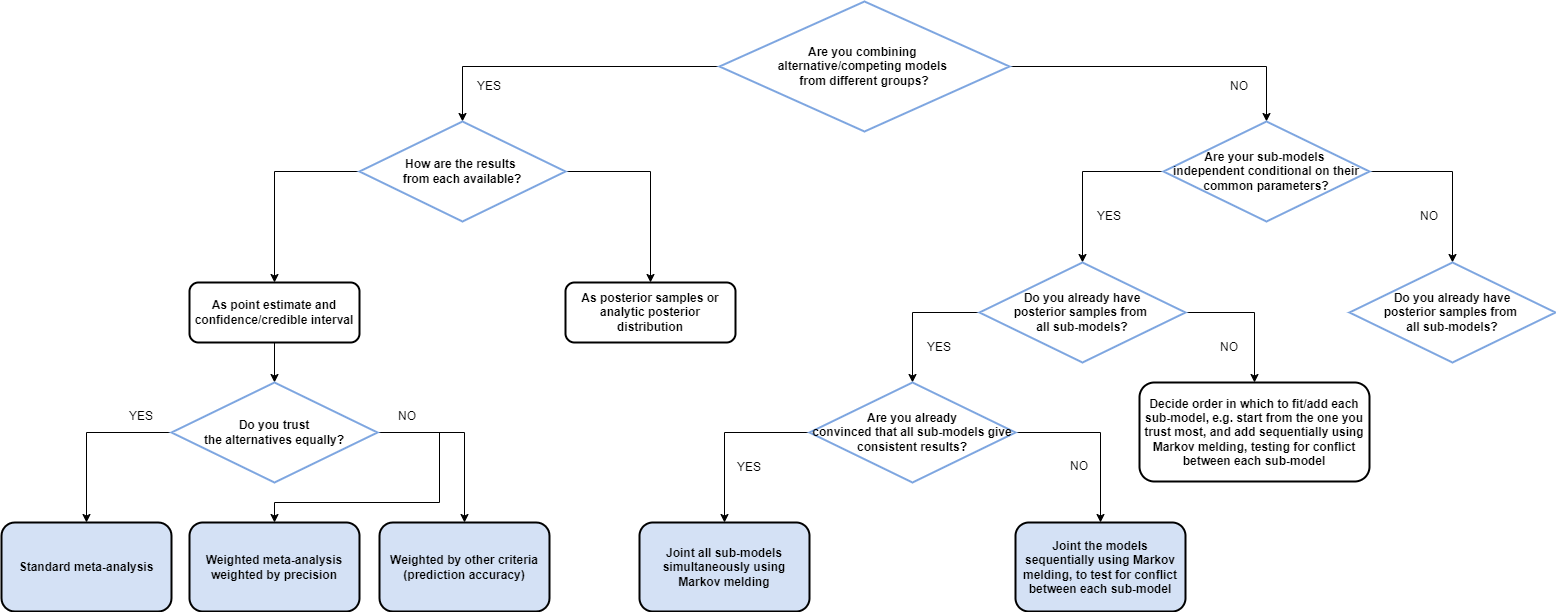
\includegraphics[width=\textwidth]{figures/integration choices decision tree.drawio.png}
    \caption{Decision tree of integration choices for integrating multiple data sources in infectious disease modelling.}
    \label{fig:integration}
\end{figure}

First stab outline 27/05
\begin{itemize}
    \item Different possible choices for integrating/ensembling inference from multiple data sources
    \begin{itemize}
        \item Full joint model fitted, regardless of whether you have already fitted separate sub-models
        \item Conditionally independent sub-models each fitted separately, then integrated
        \begin{itemize}
            \item Meta-analysis of separate estimates
            \item Weighted averaging / ensembling
            \item Markov melding
        \end{itemize}
    \end{itemize}
    \item Depends on whether you are starting from scratch, from an existing model for one data source to which you want to add others, or whether you have multiple alternative sets of existing inferences from different data sources that you want to combine
    \item General principle that modular model building (De Angelis et al, 2015; Birrell et al, 2018; Goudie et al, 2019; De Angelis \& Presanis, 2019; Gelman et al, 2020; Nicholson et al, 2022, Liu \& Goudie, 2025) is preferable, since:
    \begin{itemize}
        \item Easier to understand lack of fit, model misspecification or convergence issues from simpler sub-models individually
        \item Occam's razor - principle of parsimony, start from simplest model and build complexity up only as far as needed
        \item Adding sub-models in one at a time allows for assessment of consistency/conflict between sub-models sequentially
        \item Computational efficiency - rather than fitting full joint models after fitting the sub-models, use the posterior samples from the sub-models to obtain your full joint model (melding or ?)
    \end{itemize}
    \item Choice of likelihood function (or other objective function) and fitting choices (\ref{sec:fitting}) therefore depends on options above on where you are starting from (existing models/sub-models or from scratch)
    \item And model development is a cycle of model building and model criticism
    \begin{itemize}
        \item extension of model validation in \ref{sec:spec-validate} to multiple data sources setting
        \item detection/measurement of conflict not only between prior and data, but between data and data, or partitions of the DAG (modules) comprising different combinations of prior and data, i.e. posterior-posterior comparisons
        %\item TODO: conflict references from Fuming's literature review
    \end{itemize}
\end{itemize}

% TODO: Add practical examples of each approach
% TODO: Include decision framework for choosing integration method

\subsection{Fitting Choices}\label{sec:fitting}
% Lead: Anne Presanis, with Dhorasso and Xiahui

Inference for infectious disease models typically involves estimating a set of parameters $\theta$ from observed data $Y$, which may include case counts, hospitalizations, deaths, wastewater surveillance or other epidemiological measurements. These data are assumed to arise from a probabilistic model characterized by a likelihood function $p(Y | \theta)$ that links the parameters to the data through both an underlying transmission dynamics (represented by the process DAG in our workflow) and a noisy observation mechanism (captured by the observation DAG).  The choice of inferential approach depends on the tractability of the likelihood: 
whether $ p(Y | \theta)$ is analytically or numerically computable, intractable and requiring approximation, or entirely  unavailable (necessitating likelihood-free, simulation-based methods). This section provides a brief overview of common computational strategies, with a focus on practical considerations and current best practices.. 

\begin{figure}[htbp]
    \centering
    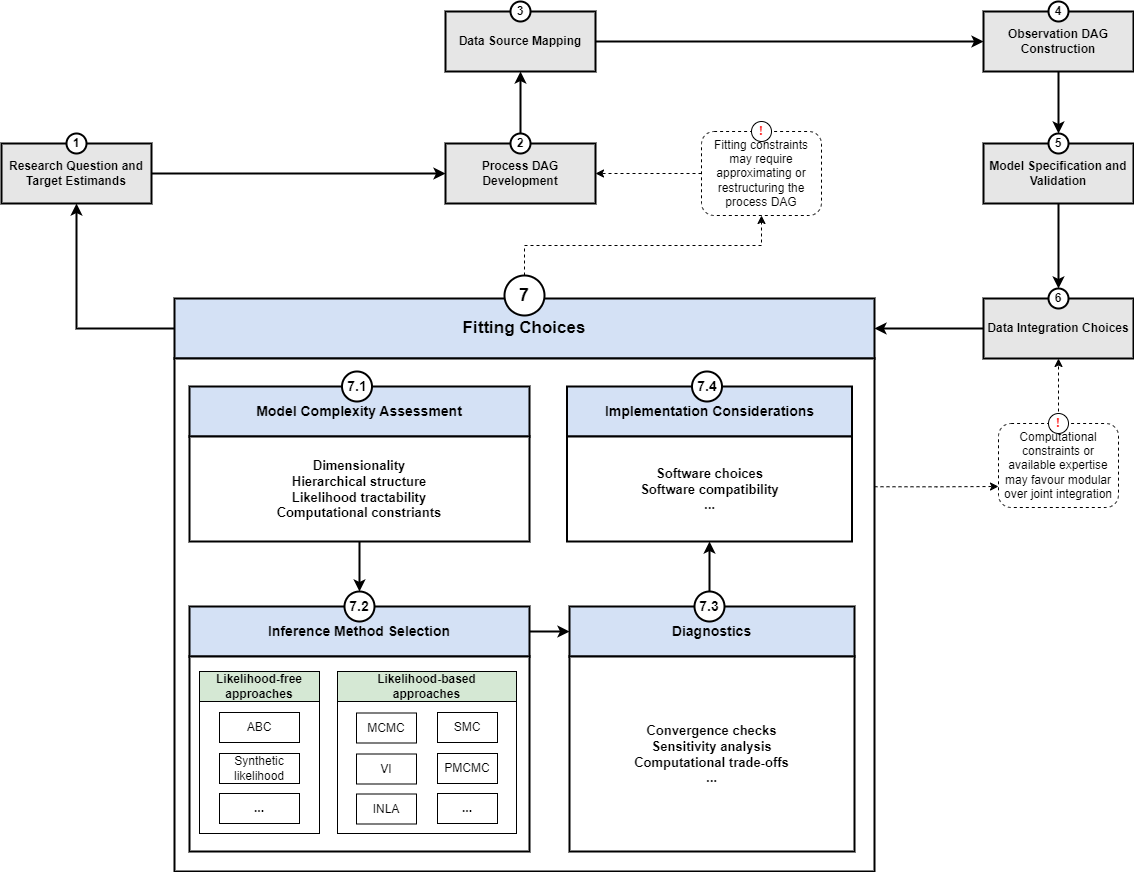
\includegraphics[width=\textwidth]{figures/Subpanel_fitting choices_v2.drawio.png}
    \caption{Fitting choices workflow for integrating multiple data sources in infectious disease modelling.}
    \label{fig:fitting}
\end{figure}

% \subsubsection{Tools for Tractable Likelihood Functions}
% % TODO: MCMC and its variants for joint models
% % TODO: Sequential Monte Carlo (SMC) approaches

% \subsubsection{Tools for Partially Tractable Likelihood Functions}
% % TODO: Particle MCMC (pMCMC) for state-space formulations
% % TODO: Variational inference (VI) and INLA for specific model classes

% \subsubsection{Tools for Intractable Likelihood Functions}
% % TODO: Approximate Bayesian Computation (ABC-MCMC, ABC-SMC)
% % TODO: ABC with history matching
% % TODO: Bayesian Synthetic Likelihood (BSL)
% % TODO: Simulation-based inference approaches



\subsubsection{Likelihood-based methods}
Likelihood-based inference encompasses frequentist and Bayesian appraoches. Classical frequentist methods such as maximum likelihood estimation (MLE)\citep{myung2003tutorial, baltazar2024maximum} and profile likelihood \citep{tonsing2018profile, plank2024structured} provide well-established tools for parameters estimation. However, here we focus mainly on Bayesian methods due to their flexibility in handling uncertainty and incorporating various sources of information.

Bayesian inference updates prior beliefs $ p(\theta)$ in light of observed data to obtain a posterior distribution, $p(\theta | Y) \propto p(Y|\theta) \,p(\theta)$. For simple models with exponential family likelihoods, conjugate priors that allow closed-form posterior solutions \citep{gelman1995bayesian,  cori2013new}. However, many infectious disease models typically involve complexities that preclude exact inference.

When the likelihood can be evaluated (up to a constant) but closed-form posteriors are unavailable, sampling-based methods, especially Markov Chain Monte Carlo (MCMC) remain the gold standard \citep{gilks1995markov, lekone2006statistical}. Common algorithms includeMetropolis–Hastings \citep{hastings1970monte} and Gibbs sampling \citep{geman1984stochastic}. For latent variable models, data-augmented MCMC introduces auxiliary states to jointly infer parameters and hidden variables \citep{o1999bayesian}. More efficient techniques such as Hamiltonian Monte Carlo (HMC) for differentiable likelihoods \citep{duane1987hybrid} and its adaptive variant No-U-Turn Sampler (NUTS) \citep{hoffman2014no, andrade2020evaluation}, leverage gradient information for faster convergence and automatic tuning. 

Alternatives to MCMC include Variational Inference (VI), which approximates the posterior by optimizing a tractable surrogate distribution, offering scalability at the cost of some bias \citep{blei2017variational, chatzilena2019contemporary}. Similarly, the Integrated Nested Laplace Approximation (INLA) 
offers a computationally efficient method for approximating posterior marginals in latent Gaussian models, without relying on sampling-based methods \citep{rue2017bayesian}.

In state-space models with high-dimensional latent state structures, the likelihood is often intractable due to the need to marginalise over latent states. Sequential Monte Carlo (SMC) methods, or particle filters, approximate the posterior using weighted particles and yield unbiased likelihood estimates \citep{doucet2001introduction}. These can be embedded within MCMC to form particle MCMC (PMCMC) \citep{andrieu2010particle, endo2019introduction} enabling joint parameter and latent state inference. Sequential Monte Carlo Squared (SMC$^2$) \citep{chopin2013smc2} extends this to fully sequential Bayesian updating as new data are accumulated.

\subsubsection{Likelihood-Free Methods}

Likelihood-based methods are powerful for parameter inference butrely on evaluating the likelihood function, which is sometimes infeasible for complex infectious disease models. Likelihood-free methods circumvent this by simulating from the model instead.

Approximate Bayesian Computation is a popular likelihood-free method that approximates the posterior distribution by accepting parameter values that generate simulated data close to the observed data under a predefined distance metric \citep{rubin1984bayesianly, tavare1997inferring, beaumont2002approximate}. While conceptually simple, the classical ABC rejection sampling is inefficient in high-dimensional settings, prompting the development of mode advanced variants. 

ABC-MCMC combines ABC with MCMC to improve sampling efficiency, especially for peaked or correlated posteriors \citep{marjoram2003markov, wegmann2009efficient, kypraios2017tutorial}. However, its performance is sensitive to the choice of tolerance thresholds and proposal distributions.

ABC-SMC further enhances efficiency by iteratively refining  tolerances and proposal distributions, adaptively focusing computational effort on high-probability regions and handling multi-modal posteriors more effectively \citep{sisson2007sequential, toni2009approximate, beaumont2009adaptive, drovandi2011likelihood}. 

When exact likelihoods are unavailable but the model can be simulated repeatedly, synthetic likelihood methods provide an alternative by approximating the likelihood via assuming Gaussian distributions for summary statistics \citep{wood2010statistical, price2018bayesian}. 

\subsubsection{Selecting the Right Tool}
% TODO: Trade-offs between computational complexity, accuracy, bias
% TODO: Interpretability and implementation ease considerations
% TODO: Decision-making frameworks for method selection

Selecting an appropriate inference method involves balancing trade-offs between computational efficiency, statistical rigor, data availability, interpretability, and model complexity \citep{funk2020choices}. Rather than adopting a universal approach, the choice should be tailored to the specific modeling context and inferential goals. 

For evolving epidemics, a key consideration is the dynamic nature of epidemic processes and data streams. As transmission rates and intervention effects change over time, and new data arrive continuously, methods that support sequential data updates, such as SMC, are generally preferred for real-time epidemic tracking \cite{birrell2020efficient, storvik2023sequential}. In contrast, MCMC-based methods, while statistically robust, are typically better suited for retrospective analyses, due to their reliance on complete datasets and high computational demands for reanalysis. 

 When computational resources are constrained, for example during real-time outbreak monitoring or when analyzing large datasets, approximate methods like VI or ABC-SMC might offer scalable alternatives \citep{chatzilena2019contemporary, engebretsen2023real}.

Beyond computational efficiency, statistical accuracy is influenced by algorithmic choices including priors distributions, tuning parameters, tolerance thresholds, and the number of particles or iterations. Full-likelihoods methods typically yield higher accuracy, subject to likelihood tractability and proper specification, whereas likelihood-free approaches often prioritise flexibility and scalability over precision \cite{alahmadi2020comparison}. 

Interpretability and ease of implementation also play a role. Certain methods integrate smoothly with probabilistic programming environments, while others may require further tuning and computational expertise. Ultimately, method selection should followa systematic decision process that considers modeling goals, urgency or latency constraints, system complexity, and available computational resources. 

Regardless of the approach chosen, model checking, sensitivity analysis, and validation are essential to ensure that inferences are not only statistically valid but also scientifically meaningful and actionable.



\subsubsection{Practical Implementation}
% Lead: Sam Abbott
% TODO: Software implementations and availability
% TODO: Diagnostic tools and convergence assessment
% TODO: Computational resource requirements
% TODO: Reference to inference subpanel workflow figure

A wide range of software tools is available to support the implementation of both likelihood-based and likelihood-free methods in infectious disease modeling. Bayesian inference platforms such as Stan, JAGS and NIMBLE are widely used for likelihood-based approaches, offering flexibility in model specification and efficient MCMC algorithms \citep{carpenter2017stan,abril2023pymc}. For more complex or high-dimensional models, Python based PyMC and Julia based Turing.jl provide probabilistic programming environments with good performance \citep{abril2023pymc,ge2018turing,fjelde2025turing}. For more scalable alternatives to MCMC, INLA is implemented in the R-INLA package \citep{martins2013bayesian} and is particularly efficient for latent Gaussian models, including spatiotemporal structures commonly used in disease mapping and surveillance. VI is also available in PyMC and Turing.jl. These implementations allow rapid inference for large datasets or real-time modelling applications.  Additionally, tools such as LibBi support SMC-based inference for state-space models and can scale to high-dimensional problems using GPU and parallel computing \citep{murray2015bayesian}. For likelihood-free methods, ABC is supported in packages like EasyABC, abc, abctools \citep{jabot2013easy,csillery2012abc,nunes2015abctools}.

Computational demands vary substantially between inference methods and can constrain the scale and complexity of implementation. MCMC methods can be computationally intensive for high-dimensional parameter spaces. VI is highly scalable and typically much faster than MCMC. However, it trades accuracy for speed and may not always be suitable where posterior uncertainty is critical. Likelihood-free methods tend to be computationally expensive because of repeated model simulation. Parallelization is essential and HPC resources are often required for large-scale studies. 

\section{Case Studies}
% Lead: Anne Cori

\subsection{Overview}

We demonstrate our iterative workflow through four progressive case studies, each building complexity whilst showing different integration choices and methodological considerations.
All case studies share a common estimand -- the time-varying reproduction number ($R_t$) -- while the final case study has the overdispersion parameter ($k$) as an additional estimand. The case studies use SARS-CoV-2 outbreak data to leverage expert survey evidence on data source characteristics.
Each case study follows our complete workflow framework, demonstrating how adding more data sources enables analyses to answer questions that would otherwise require strong assumptions.

The progression between case studies illustrates key principles: case counts are often used to monitor transmissibiliy over time but require assumptions on the fraction of infections reported (CS0); data on deaths can eliminate reporting fraction assumptions that beset case-only analyses (if the case fatality ratio is known, CS1); wastewater data eliminates testing bias inherent in symptomatic surveillance (but is limited by uncertainty in the average shedding rate per infected individual, CS2); individual-level data enables direct overdispersion estimation without distributional assumptions (CS3).
Implementation choices reflect practical considerations including available expertise, computational resources, time availability, and model complexity trade-offs, whilst generally favouring efficient methods like NUTS where applicable.

TODO: need to add something on data source mapping which all the case studies will draw from: what data are available that may inform Rt and superspreading estimates? (Can draw from the survey and Anne C's slides at CIRM). What are their pluses and minuses (if we cannot do the full mapping from survey we can still discuss - otherwise refer to that section).

\subsection{Data survey}

\paragraph{}We conducted a survey of participants at a workshop on the role of modelling for epidemic surveilllance (see supplementary material) to systematically evaluate different data sources for infectious disease modelling.
Our survey may help practitioners rate different data sources on quality, timeliness, and usefulness for modelling SARS-CoV-2. We pooled expert opinions to create visual comparisons showing trade-offs between different data types, making it easier to assess which data to use when estimating transmissibility and identifying when different data sources might conflict.

\paragraph{}To systematically identify potential biases across multiple data sources, we developed a structured questionnaire. As our group comprised of researchers from diverse disciplinary backgrounds who have experience in working with various sources of data, the questionnaire design process was shaped by a broad range of perspectives. Our main goal in developing this questionnaire was to enable a visual and comparative assessment of the data source strengths. Therefore, we agreed upon six primary evaluation categories, which we have already discussed in Section XXXX (data characteristics): basic metadata, scope, resolution, data quality, data utility, and practical considerations. Each category was further subdivided into specific subcategories, which allowed respondents to provide input within prespecified ordinal-scale categories, numerical scale (ranging from 0 to 5), and qualitative responses through free-text. We expected this questionnaire structure to facilitate multidimensional characterisation of the data sources, which could in turn support more informed decisions in data selection and integration. 

\paragraph{}Within the basic \textit{metadata} section, predefined options included time-series data, hospitalisation time-series data, wastewater data, or other, with the latter allowing specification of alternative sources of data. This first classification of data served as a foundation for subsequent evaluations, ensuring that the responses were contextualised according to the nature of the data sources under consideration. Furthermore, within this section, respondents were asked to provide a free-text description of the data content, as well as to indicate the primary purpose of the data collection, whether for clinical management or other objectives. These inputs were intended to capture essential basic information of the data source that could affect the interpretation and applicability. 

\paragraph{}Next, the \textit{scope} section of the questionnaire focused on the characteristics of the population represented in the data. Respondents were first asked to specify, via free-text, the source population---the broader population from which the data were sampled. They were also asked to identify the target population, selecting from pre-defined categories such as age-specific, risk-specific, convenience samples, geographic subsets, health-care related populations, the entire population, or other (via free-text option). Additional questions addressed whether the population was stratified by demographic, clinical, or other relevant factors. The respondents were asked to indicate the type of data collection--routine, triggered, or one-off. If the data collection was triggered, further clarification was requested regarding the nature of the trigger (for example, exceeding a specific threshold or the detection of a new pathogen/ variant). 

\paragraph{}The \textit{resolution} section of the questionnaire addressed the level of detail available in each data source. Respondents were first asked to indicate whether the data were collected at the individual level or in an aggregated form. For data with a temporal component, additional questions captured the frequency of the data collection (continuously, daily, weekly, etc.), the frequency of reporting (continuously, daily, weekly, etc.), and the period covered (early outbreak, peak, endemic phase, continuous monitoring or other). If the data included spatial information, the respondents were asked to specify the lowest spatial resolution available, with options to select from international, national, regional, local, or hyperlocal levels. Finally, the respondents were asked to rate, on a scale from 0 to 5, the completeness of coverage across the intended geographical areas. These questions were aimed to asses the the data granularity as well as comprehensive from both a temporal and spatial dimensions. 

\paragraph{}The \textit{data quality} section focused on evaluating the reliability and the trustworthiness of each dataset. Respondents were first invited to provide a free-text description of the perceived quality of the data. They were then asked to asses whether the case definitions used were standardized--across time, space or both--by assigning a score on the scale from 1 to 5. The same numerical scale was used to evaluate key factors of measurement quality, such as sensitivity and specificity of any diagnostic test that was used, the potential for unexplained variability, and the extent of reporting delays. To further explore the potential sources of bias, the respondents were gain invited to provide a description of potential biases, followed by assigning a score from 1 to 5 on issues such as missing data, censoring, truncation, and selection (underrespresntative sampling relative to the target population). The respondents were also asked to asses the potential for selection bias by identifying contributing factors such as ascertainment or under reporting, location-specific observation, and socio-economic infleunecs [these are not all the factors in the questionnaire]. Finally, the respondents were asked to characterise the bias by giving a score from a 1 to 5 scale for biases to vary over time and the direction of bias. 

\paragraph{} The \textit{data utility} section was used to evaluate transmission metrics that the data can inform, and how these metrics could be derived. Respondents were asked to identify which epidemiological targets (such as basic reproduction number, incidence, prevalence, etc) and for each selected metric, they are prompted to specify whether it could be calculated directly, indirectly, or cannot be informed by the dataset. To assess the generalizability of the data, the respondents were asked to rate, on a scale of 1 to 5, the extent to which the information can be generalised to a general population. In cases where generalisations were not possible, the respondents were asked to provide the reason in the form of free text to understand the dataset's applicability. 

\paragraph{}The \textit{practical considerations} section addressed the feasibility and operational aspects of using a dataset. Respondents were asked to indicate the scalability of the data source by selecting from predefined options such as independent, sub-linear, or other relevant categories. They were then asked to rate, on a scale of 1 to 5, key dimensions: sustainability, cost, accessibility, and linkage potential. For datasets that were linked to other sources of data, the respondents are asked to choose the types of data linked, using the same classification we used at the beginning of the questionnaire.  Additionally, the respondents were asked to rate the level of structure within the dataset and the generalisability of the findings to other pathogens, both on a scale of 1 to 5. If the data can be generalisable, a free-text space was provided to list the specific pathogen. 


\begin{itemize}
    \item The Fellowship assembled
    \item We made a survey
    \item Here is that survey
    \item We found our inner power
    \item That power was data analysis of our data survey
    \item We now refer back to this power throughout the case studies.
\end{itemize}


\subsection{Case Study 0: Single-Source Baseline (Cases Only)}


The research question for this case study (and case studies 1 and 2) is: what is the time-varying reproduction number $R_t$ during this outbreak period?
The objective of this case study is to showcase the workflow and explore some of the assumptions and modelling and fitting choices underlying estimation of $R_t$ from a single time series of case incidence.



%\textbf{Workflow Demonstration:}
%\begin{enumerate}
%    \item \textbf{Process DAG:} Simple renewal equation linking Rt to case incidence through generation time distribution, incorporating overdispersion via negative binomial model
%    \item \textbf{Data Source Mapping:} Case incidence time series selected based on expert survey ratings showing high timeliness but moderate precision due to testing policy effects
%    \item \textbf{Observation DAG:} Reporting delays, underascertainment fraction, weekend reporting effects
%    \item \textbf{Integration Choice:} Single source (no integration required)
%    \item \textbf{Implementation:} NUTS sampling of renewal equation with negative binomial observation model, chosen for computational efficiency and robust performance
%\end{enumerate}

%\textbf{Key Limitation:} Establishes baseline uncertainty but requires strong assumptions about generation time distribution and reporting fraction, highlighting assumption-dependent limitations that motivate multi-source approaches.

\textbf{Workflow Demonstration:}
\begin{enumerate}
    \item \textbf{Process model}: We consider three variants of the renewal process model for the number of new infections $I_t$ on day $t$, which is influenced by the instantaneous reproduction number $R_t$ on day $t$, and the generation time (GT) distribution, which we assume to be fixed. The three model variants are:
\begin{itemize}
    \item[P1.] No variance in daily infection incidence (deterministic)
    \begin{equation} \label{eq:infections_P1}
        I_t = R_t \sum_{s=1}^\infty I_{t-s}w_s 
    \end{equation}
    \item[P2.] Poisson-distributed daily infection incidence.
        \begin{equation} \label{eq:infections_P2}
        I_t \sim \mathrm{Poiss}\left( R_t \sum_{s=1}^\infty I_{t-s}w_s  \right)
    \end{equation}
    \item[P3.] Negative binomially distributed daily infection incidence. 
            \begin{equation} \label{eq:infections_P3}
        I_t \sim \mathrm{NegBin}\left( R_t \sum_{s=1}^\infty I_{t-s}w_s, k  \right)
    \end{equation}
\end{itemize}
where $w_s$ is the probability mass function for the GT distribution and $k$ is the dispersion parameter. 
The process DAGs for these three models are shown in Figure \ref{fig:CS0_DAGs}.

 
% **********MJP: I think we (SA+AC+MP) agreed this is now covered already in the "Data sources and characteristics" section. But having read ahead to CS1 and 2, maybe it is useful to provide a brief remark here to illustrate the owrkflow? 
\item \textbf{Data source mapping}: Case incidence data is typically readily available with very frequent (often daily) updates and high timeliness. However, it is an imperfect and potentially biased proxy for infection incidence, and is dependent on testing patterns and lab processing and reporting timeliness. 


\item \textbf{Observation model}: The observation model relates the observed data (here daily case incidence) with underlying latent variables (here daily infection incidence). 
This requires assumptions to be made about underreporting (what fraction of infections are detected cases), reporting delays (time between infection and a case being detected and reported), and random noise (typically used to capture other things not explicitly specified in the model).

Alternative versions of the observation model can be considered, which either ignore or include each of these three aspects. This leads to $2^3=8$ possible observation models, each of which has an associated DAG (although some DAGs may be the same).
We refer to these models as $O_{000}$ (for the simplest observation model not modelling any of the above) to $O_{111}$ (for the most comprehensive accounting for all three observation features).

\item \textbf{Fitting and integration approach}: As there is only one data source in this case study, no decisions about what and how to integrate multiple sources are needed. The choice of fitting method may depend on considerations such as analytical tractability of the combined process and observation model, computational complexity and speed of computation relative to the time available, and identifiability issues. 
 
% \begin{itemize}
%     \item Fitting choice discussion points to add:
%     \item Analytically tractable or not. Depends on the specific choices of PRIOR, P and O, the resulting model has an analytic formulation or not which guides choice here
%     \item Identifiability issues
%     \item Computational complexity / speed of computation
% \end{itemize}

One scenario requiring integration though would be model ensembling, where multiple estimates of the target estimand (in this case $R_t$) are produced by different groups or methods based on the same data, and synthesised into a combined estimate. [***Link to SPI-M paper from Oxford]. In this context, it may be desirable to align the assumptions made by different models, for example about the GT distribution or the temporal smoothness in $R_t$, to ensure that estimates from the different models are  comparable [***Johannes’ paper].

\item \textbf{Implementation}: Implementation requires selection of one process model, one observation model and one fitting and integration method (which will depend on the choice of process and observation model as described above). For this case study, combinations of the 3 process models and 8 observation models give 24 possible models, on top of which alternative fitting methods can be chosen for each. Here, we give a few examples from the literature:
\begin{itemize}
    \item EpiEstim. This method assumes Poisson distributed infections, no underreporting, no delays in reporting, and no observation noise \citep{cori2013new}. In our categorisation, this corresponds to process model P2 and observation model $O_{000}$. The model is fitted by calculating an analytic posterior distribution for $R_t$ from a conjugate prior, which is fast and computationally efficient. 
    \item EpiNow2 [***may need to specify a version]. This method assumes deterministic infection incidence with no underreporting, but with delays and random observation noise. In our categorisation, this corresponds $P_1-O_{011}$. This is fitted using XXX.
    \item Epidemia or EpiMap for NB process – TODO: check what they do!
\end{itemize}

Other possible choices of fitting methods that could be considered / why not (refer to relevant section in the overall framework description)
 \end{enumerate}
 
% TODO: add a Figure. This will be A visual of jigsaw puzzle presenting a library of P (process models), O (observation models) and F (fitting methods). In multi-data ones we will need to add an I (integration method) too.
% Example choices of EpiEstim and EpiNow2 for example (as above). Prototype figure below

% \begin{figure}
% 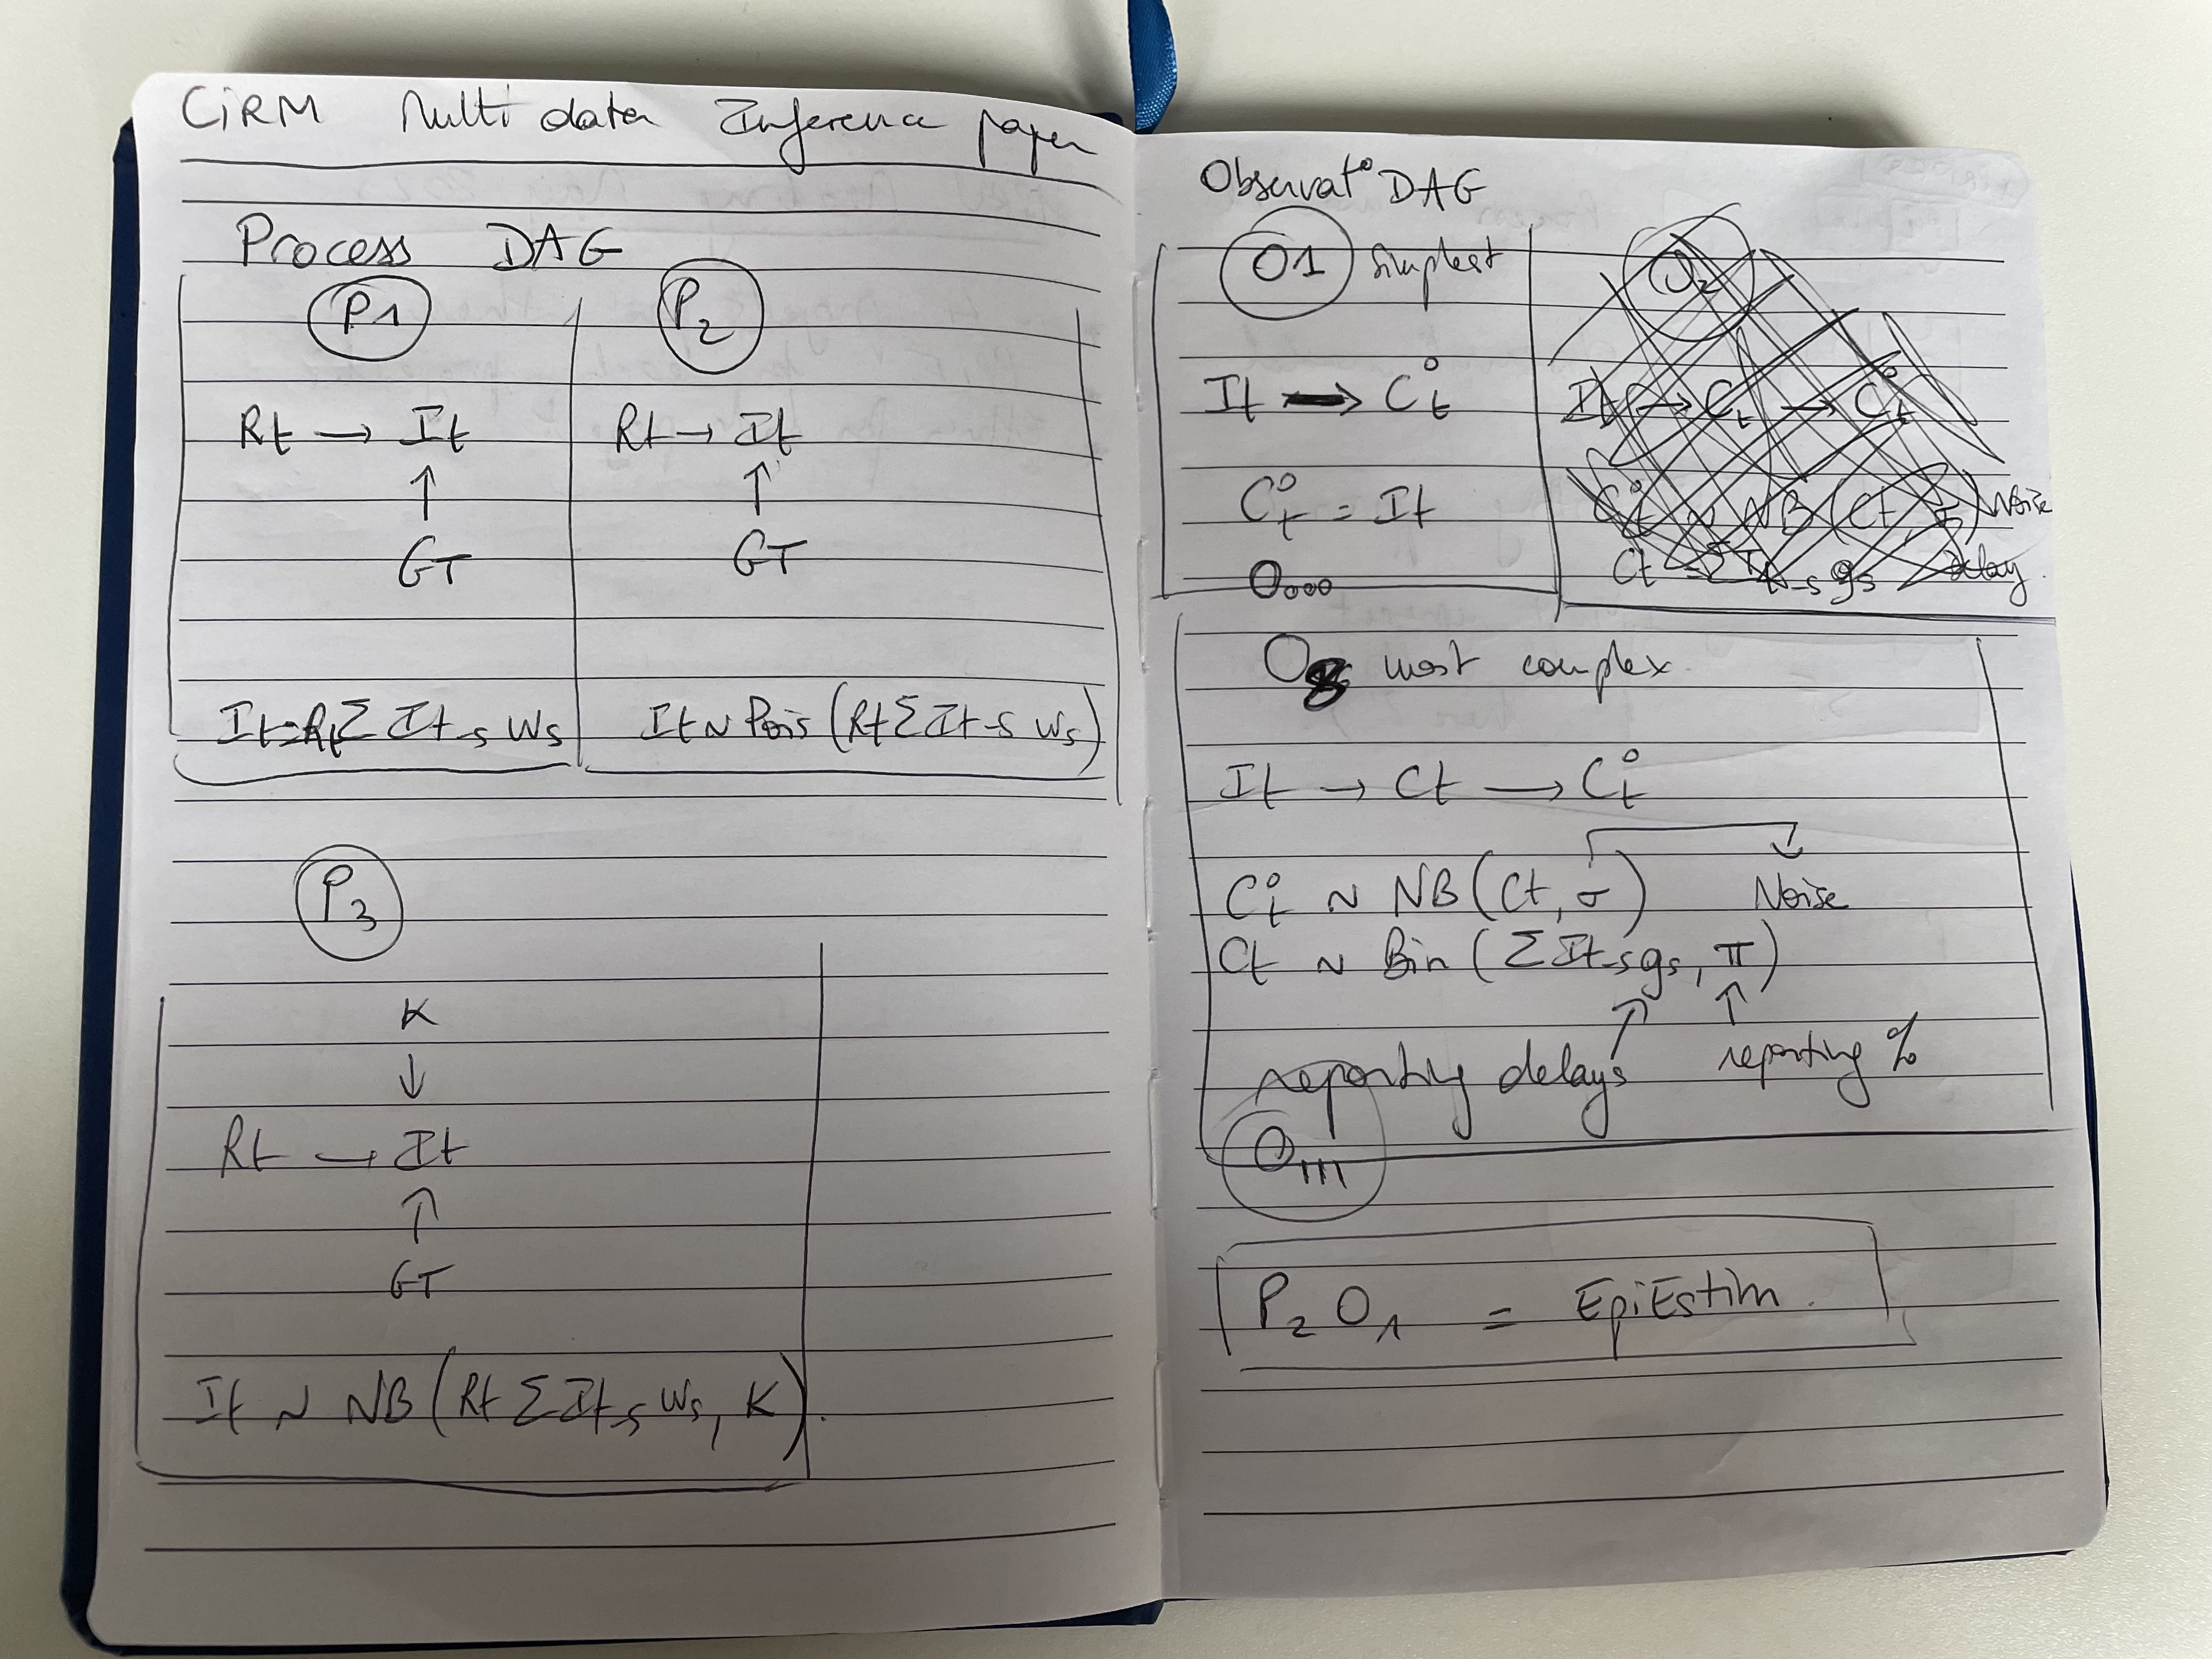
\includegraphics[width=0.75\textwidth]{figures/cs0_diagram1.jpg}
% \label{fig:CS0_DAGs}
% \caption{Process model DAGs for case study 0.}
% \end{figure}

% 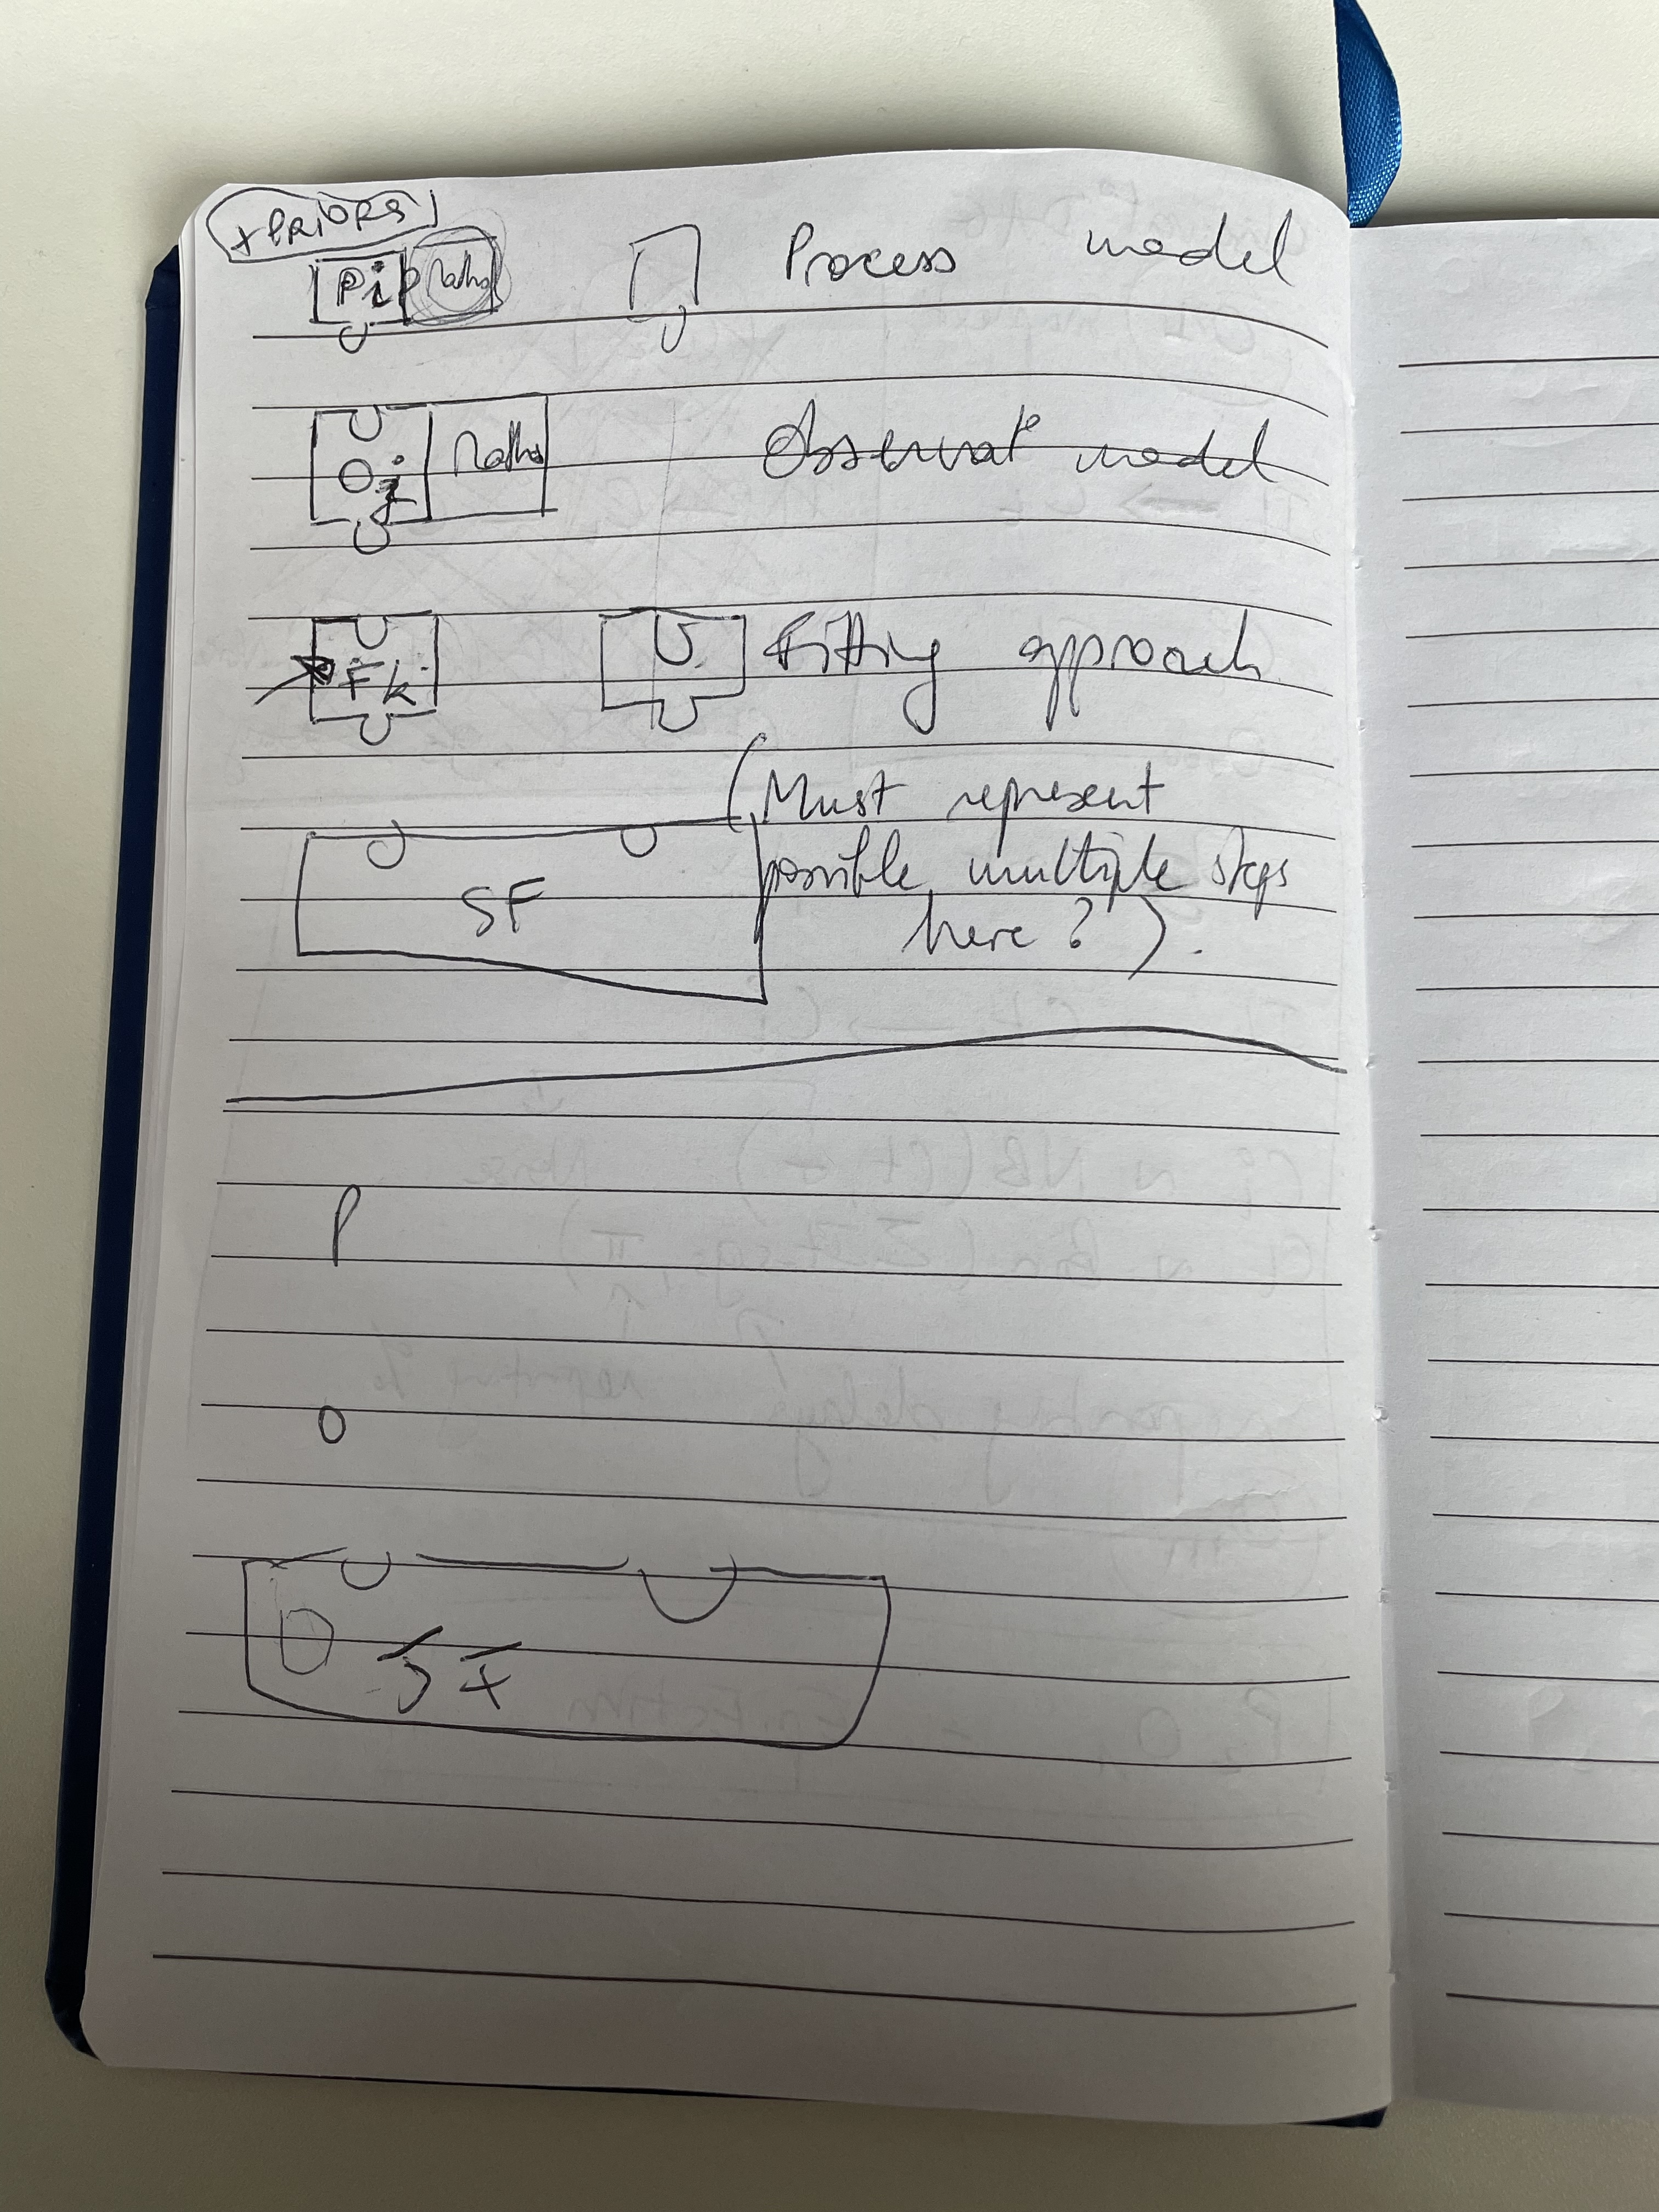
\includegraphics[width=0.75\textwidth]{figures/cs0_diagram2.jpg}

\begin{figure}[htbp]
    \centering
    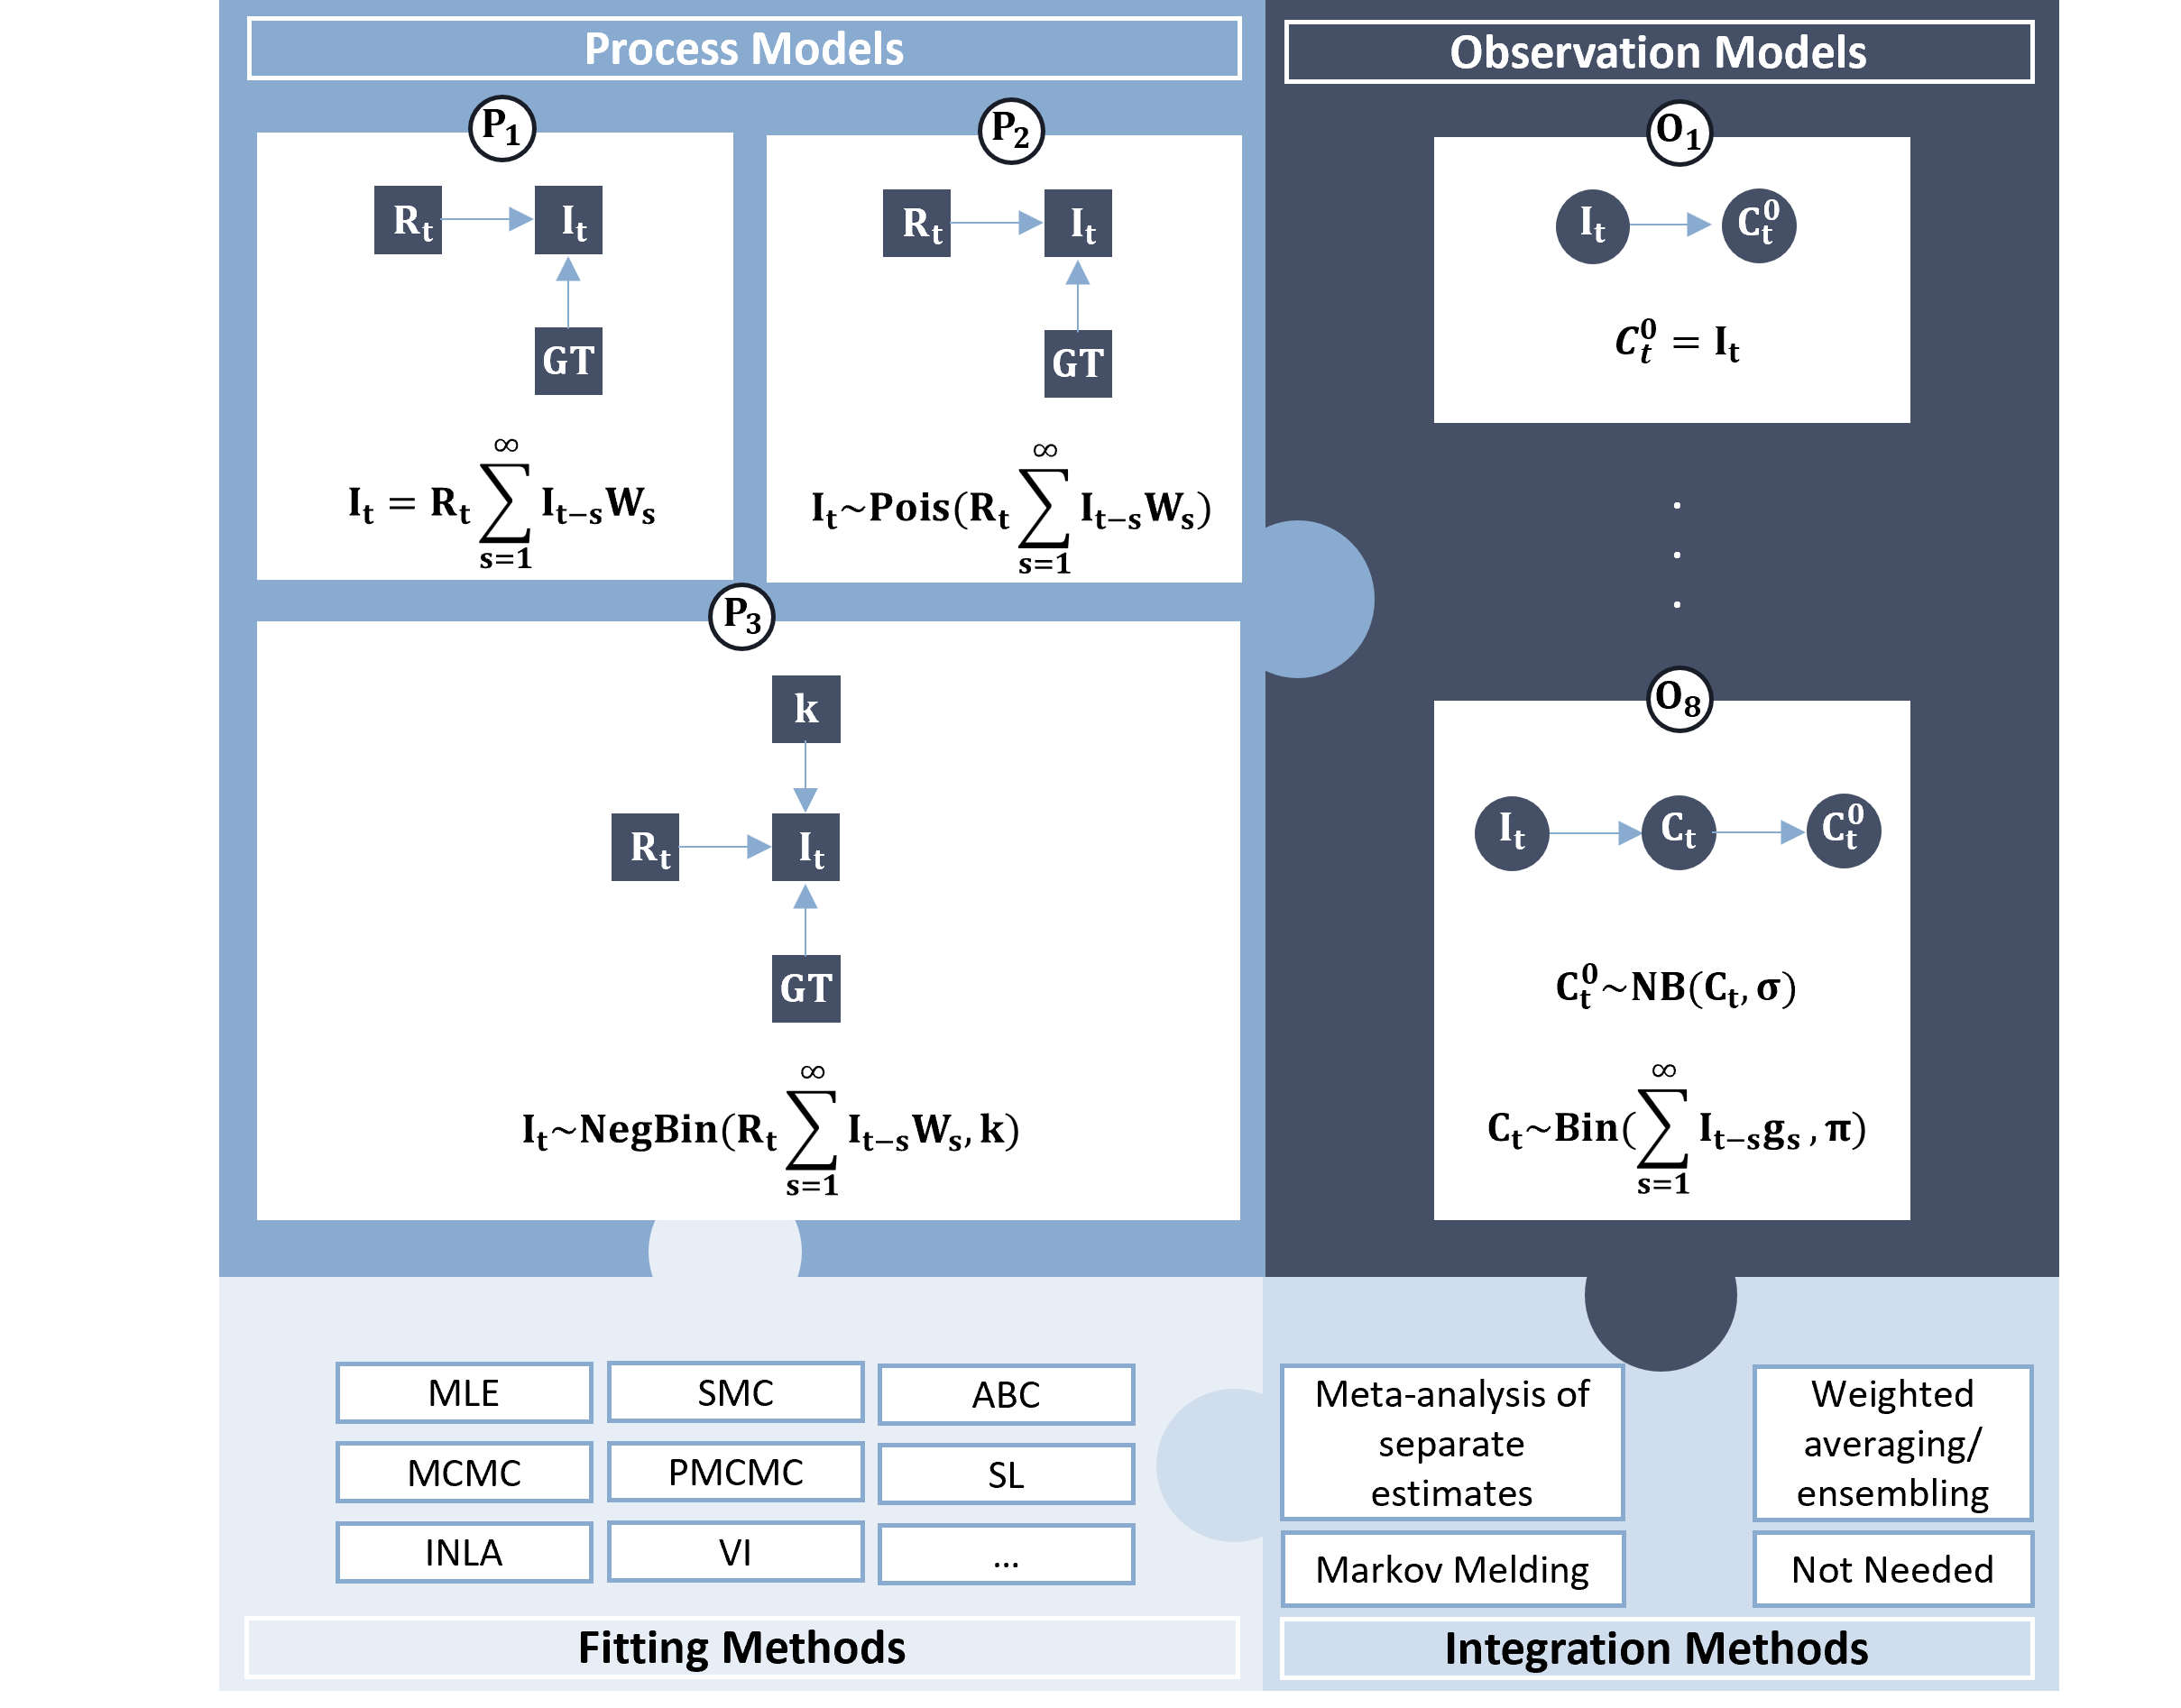
\includegraphics[width=\textwidth]{figures/Case study puzzle.png}
    \caption{A visual of jigsaw puzzle presenting a library of process models, observation models, integration methods, and fitting methods.}
    \label{fig:case_study_visual}
\end{figure}

\textbf{Question to Anne P} – can we write the model (e.g. assuming Poisson likelihood) as part of the DAG or is that something separate? If separate then we should make it clear throughout that the DAG isn’t the full model spec.

Different approaches have different strengths and limitations. For example, the key strength of EpiEstim is computational speed, whereas its key weaknesses are ignoring underreporting and reporting delays. The former may be less important in contexts where the reporting fraction can reasonably be assumed to be steady over the time period of interest. Furthermore, any change in reporting fraction will not be identifiable from a case time series alone, so it would not be sensible to attempt to estimate this in this example. EpiNow2 overcomes some of these weaknesses, at the cost of increased computational complexity. The more appropriate option may depend on the balance between need for timely estimates (e.g. for modelling an outbreak in real-time) and the realism of the associated assumptions. 

A common weakness of all the models outlined above is that they assume the GT distribution is constant and perfectly known. Some approaches (e.g. some versions of EpiEstim) extend the approach to relax this assumption (see also Case Study 4).
 
% \textbf{Next steps}:
% \begin{itemize}
%     \item feedback from others on case study 0
%     \item Anne C to draft similar case study 1 (cases + deaths)
%     \item Someone with skills to make nice picture of my horrific handwritten plots
% \end{itemize}




\subsection{Case Study 1: Two-Source Integration (Cases and Deaths)}

The target estimand for this case study is the same as in case study 0 ($R_t$). The objective of this case study is to illustrate the process and challenges of adding an additional data stream (in this case death data), and to explore how this can improve $R_t$ estimation and reduce assumption dependence.

\textbf{Workflow Demonstration:}
\begin{enumerate}
    \item \textbf{Process model iteration:} The number of deaths $D_t$ on day $t$ depends on the time series of infections up to day $t$, the infection-fatality ratio $p_d$, and the distribution $v_s$ of time ($s$) from infection to death. This can be represented in the process DAG (Figure X) and by the following convolution equation:
    \begin{equation} \label{eq:deaths}
        D_t \sim \mathrm{Poiss}\left(p_d \sum_{s=1}^\infty I_{t-s}v_s \right)
    \end{equation}
    Other process models for deaths are possible, for example using a multinomial model for the number of deaths occurring on day $s+k$ due to infections on day $s$ ($k=1,2,\ldots$). However, the Poisson model is a good approximation provided $p_d\ll 1$. This formulationassumes that the probability $p_d$ of an infection resulting in death and the distribution of time from infection to death $v_s$ are fixed and known.
    
    Eq. \eqref{eq:deaths} provides a model for the time series of daily deaths $D_t$ conditional on the time series of daily infections $I_t$ and would typically be used in combination with one of Eqs. \eqref{eq:infections_P1}--\eqref{eq:infections_P3} that describe the dynamics of infections to produce a joint model for infections and deaths. 
    \item \textbf{Data source mapping:} Expert survey shows deaths have higher reporting delays but lower noise (e.g. due to "day-of-the-week" reporting effects), higher ascertainment, and less policy dependence than cases (e.g. due to changing testing patterns).
    \item \textbf{Observation model:} Similar to the different choices of observation model for cases described in case study 0 (and still relevant to this case study), the observation model for deaths could include underreporting, reporting delays, and random noise. In jurisdictions with comprehensive death records, it may be reasonable to assume all deaths are reported and there is no additional observation noise, but it may still be important to account for observation delays, for example delay from date of occurrence to date of registration. This would corresponds to observation model $O_{010}$.
    \item \textbf{Integration choice:} 
       Two different approaches are possible for integration: (1) a joint model including both cases and deaths with a shared latent state $R_t$; (2) separate models for cases and deaths, resulting in two estimates for $R_t$ to be combined via a weighted ensemble. 
       
       As outlined above, we recommend fitting separate models to the two time series initially, to understand their behaviour and reveal whether they lead to consistent or conflicting estimates of $R_t$. Where inconsistent results emerge, these could lead to refinement of the model (i.e. going back to step 1); for example should $R_t$ estimates show similar trends but shifted in time, assumptions about delays may be revisited. Once this has been done, it may be desirable to combine the results into a single estimate by ensembling, or to fit a joint model that produces a single estimate from both data sources.  
       
    \item \textbf{Implementation:} For separate models, a good choice would be NUTS for estimation, followed by Markov melding to ensemble the results from the two models. For a joint model, a numerical method such as particle MCMC would likely be needed due to the state-space formulation complexity.

    \textcolor{red}{I think we should add some examples from the literature here. Just adding some notes for now:} 1) EpiNow2 seems to allow fitting jointly to cases and deaths: \url{https://wellcomeopenresearch.org/articles/5-112} - they use P1 for infections, but not very clear about cases and deaths - would need Sam's help here 2) this has several models based just on deaths - the last one uses cases and deaths but I don't think has a mechanisms for cases changing over time \url{https://journals.plos.org/plosone/article?id=10.1371/journal.pone.0286199} 3) I think Epidemic uses only deaths actually \url{https://static-content.springer.com/esm/art%3A10.1038%2Fs41586-020-2405-7/MediaObjects/41586_2020_2405_MOESM1_ESM.pdf}

    \end{enumerate}

\textbf{Key Insight:} In case study 0 using data on cases alone, the case ascertainment rate (i.e. the proportion of infections that are reported as cases) was non-identifiable and had to be assumed. Including data on deaths, if the infection-fatality ratio is known, means that the case ascertainment rate could be included as a target for estimation. However, this requires assumptions about the distribution of time from infection to death, demonstrating how additional data sources can shift rather than eliminate the need for modelling assumptions.




\subsection{Case Study 2: Three-Source Integration (Cases, Deaths and Wastewater)}

The target estimand for this case study is the same as in the previous case studies ($R_t$). The objective of this case study is to explore ways of handling conflicting signals between data sources and incorporating complex observation processes.

\textbf{Workflow Demonstration:}
\begin{enumerate}
    \item \textbf{Process model iteration:} 
    Suppose that the average concentration $W_t$ of pathogen RNA in wastewater on day $t$ depends on the time series of infections up to day $t$ and the average amount of pathogen RNA that an individual sheds into wastewater $s$ days after being infected ($s=1,2,\ldots$). This can be represented in the process DAG (Figure X) and by the following equation for $W_t$:
    \begin{equation} \label{eq:wastewater}
        W_t \sim \Gamma\left( \frac{\alpha}{N}\sum_{s=1}^\infty I_{t-s}u_s, b   \right)
    \end{equation}
    where $\alpha>0$ is a constant representing the average total amount of pathogen RNA that an infected individual sheds over the course of their infection, $N$ is the population size, $u_s$ is the average shedding rate $s$ days after infection normalised such that $\sum_{s=1}^\infty u_s=1$, and $\Gamma(\mu,b)$ denotes a gamma distribution with mean $\mu$ and shape $b$. This was similar to the wastewater model used by REF; other choices of continuous non-negative-valued distributions are possible for $W_t$ such as a log-normal distribution.

    Eq. \eqref{eq:wastewater} would be combined with one of Eqs. \eqref{eq:infections_P1}--\eqref{eq:infections_P3} for infections and with Eq. \eqref{eq:deaths} for deaths.
    \item \textbf{Data Source Mapping:} Wastewater offers population-level signal independent of testing biases, with moderate timeliness but requiring environmental expertise. It could also be affected by unknown changes in the average shedding rate $\alpha$ over time. 
    \item \textbf{Observation model:} 
   Wastewater samples are typically collected at some cadence from one or more sampling sites, and the concentration of pathogen RNA in the samples is quantified via PCR testing. 
   The existence of multiple sites with different catchments populations and non-contemporaneous sampling frequencies complicates the interpretation of quantitative wastewater data, which can be modelled at varying levels of complexity.  
   
    Here, we assume that a quantitative wastewater measurement $W_t$ drawn according to Eq. \eqref{eq:wastewater}, either from a single representative site or a suitable average of multiple sites, is available on some subset of days $t$. 
    More complex models could incorporate other factors such as individual-level and site-level variation, catchment population dynamics, spatial heterogeneity, different sampling methods, and environmental degradation.
    \item \textbf{Integration choice:} As in case study 1, we recommend that a modular approach with sequential consistency assessment is initially taken to detect and resolve data source conflicts. For example, a time lag in estimates of $R_t$ from wastewater data alone relative to estimates of $R_t$ from cases alone could suggest misspecification of the shedding rate distribution $u_s$. Once conflicts have been identified and resolved, independent estimates of $R_t$ from these models could be combined by ensembling, or a joint model could be fitted with a shared $R_t$ state. 
    \item \textbf{Implementation:} ABC-SMC for wastewater sub-model due to likelihood intractability, reflecting available environmental modelling expertise; NUTS for case/death models. For a joint model, a method like particle MCMC would likely be needed due to the state-space complexity.
\end{enumerate}

\textbf{Key insight:} Wastewater data enables trend estimation independent of shifts in testing patterns, but requires assumptions about the shedding, environmental and sampling processes. A modular approach facilitates conflict detection between data sources. The average shedding rate $\alpha$ is typically unknown and non-identifiable from available data. Similar to the unknown case ascertainment rate in case study 0, estimates of $R_t$ will be insensitive to the value of $\alpha$ provided it does not change over time. However, changes in the average shedding rate due to, for example, pathogenic evolution or changes in population immunity, would invalidate this simple model and require a more nuanced approach.  



\subsection{Case Study 3: Individual-Level Data (Cases and Transmission Pairs)}

The research question for this case study is what is the time-varying reproduction number $R_t$ and how much heterogeneity is there in individual transmission rates? The latter is captured by the additional estimand $k$, representing the dispersion in the distribution of the number of secondary cases per index case. The objective of this case study is to illustrate how different types of data (time series count data and individual-level data from contact tracing records) can be combined to enable estimation of additional quantities. 


\textbf{Workflow Demonstration:}
\begin{enumerate}
    \item \textbf{Process model iteration:} Including information on individual-level variables, as opposed to just aggregate daily counts, requires a shift from the population-level renewal equation (Eqs. \eqref{eq:infections_P1}--\eqref{eq:infections_P3}) to an individual-level model which explicitly represents the transmission tree. A DAG for this type of model is shown in Figure \ref{fig:CS3_DAG}. Mathematically, this can be expressed in terms of the number $N_{i,t}$ of people newly infected by individual $i$ on day $t$:
    \begin{equation} \label{eq:individual_level}
    N_{i,t} \sim \mathrm{Poiss} \left( R_t w_{t-T_i} Y_i\right)
    \end{equation}
    where $T_i$ is the infection time of individual $i$ and $Y_i$ is a continuous, non-negative random variable with mean $1$, representing the relative transmission rate of individual $i$ (which may capture a combination of biological and social factors). This formulation provides a way to explicitly simulate the full epidemic transmission tree.  In the special case where $Var(Y)=0$ (i.e. there is no individual-level heterogeneity), the total number of new infections on day $t$ ($I_t$) reduces to Eq. \eqref{eq:infections_P2}. The model has the property that the total number of secondary cases $Z(t)$ arising from an individual infected on day $T$ and with given individual-level transmission parameter $Y$ is
    \begin{equation}
       Z(t) \ | \ Y \sim \mathrm{Poiss}\left( Y \tilde{R}(t)\right)
    \end{equation}
    where $\tilde{R}(t)= \sum_s R_{t+s} w_s$ is the effective reproduction number averaged over the infectious period of an individual who was infected on day $t$. If $Y$ has a gamma distribution, i.e. $Y_i\sim \Gamma(1,k)$ for some dispersion parameter $k$, then the number of secondary cases caused by a randomly selected individual infected on day $t$ is
     \begin{equation} \label{eq:offspring_dist}
        Z(t) \sim \mathrm{NegBin}\left( \tilde{R}(t), k\right)
    \end{equation}   

    Note that this model assumes that the relative infectiousness profile over time $w_s$ is fixed and identical for all individuals. This is a reasonable starting assumption, but it may be important to relax this in some situations, for example to model the impact of quarantine and isolation measures on individuals identified by contact tracing.
    \item \textbf{Data source mapping:} Contact tracing records identify transmission pairs, which contain information about heterogeneity in transmission patterns, contingent on contact tracing system quality. The smaller the dispersion parameter $k$, the more variance would be expected in the distribution of the number of secondary infections per index case.
    \item \textbf{Observation model:} Observation models for reported daily case counts, daily deaths and wastewater samples as outlined previously would be coupled with a model for the probability of observing model a given set of transmission pairs, for a given level of contact tracing coverage and delay effects. Eq. \eqref{eq:offspring_dist} can be used to derive the likelihood of a person who was infected on day $t$ causing a total of $n$ secondary infections, for a given value of the parameter $k$ and the state variables $R_{t+s}$ ($s=1,2,\ldots$). 
    \item \textbf{Integration choice:} A hierarchical model linking individual transmission events to population-level reproduction number would be a suitable framework.
    \item \textbf{Implementation:} NUTS with data augmentation for unobserved transmissions, chosen for efficient handling of discrete latent variables. Alternative a method such as particle marginal Metropolis Hastings could be used to used to estimate the time-varying reproduction number $R_t$ and the fixed parameter $k$ in a hierarchical manner (but may be computationally slow). 
\end{enumerate}

\textbf{Key Insight:} Individual-level data enables direct overdispersion estimation without distributional assumptions but requires contact tracing completeness assumptions. This shows how data granularity can fundamentally change model structure and inference requirements.

\begin{figure}
\centering
(a) \\
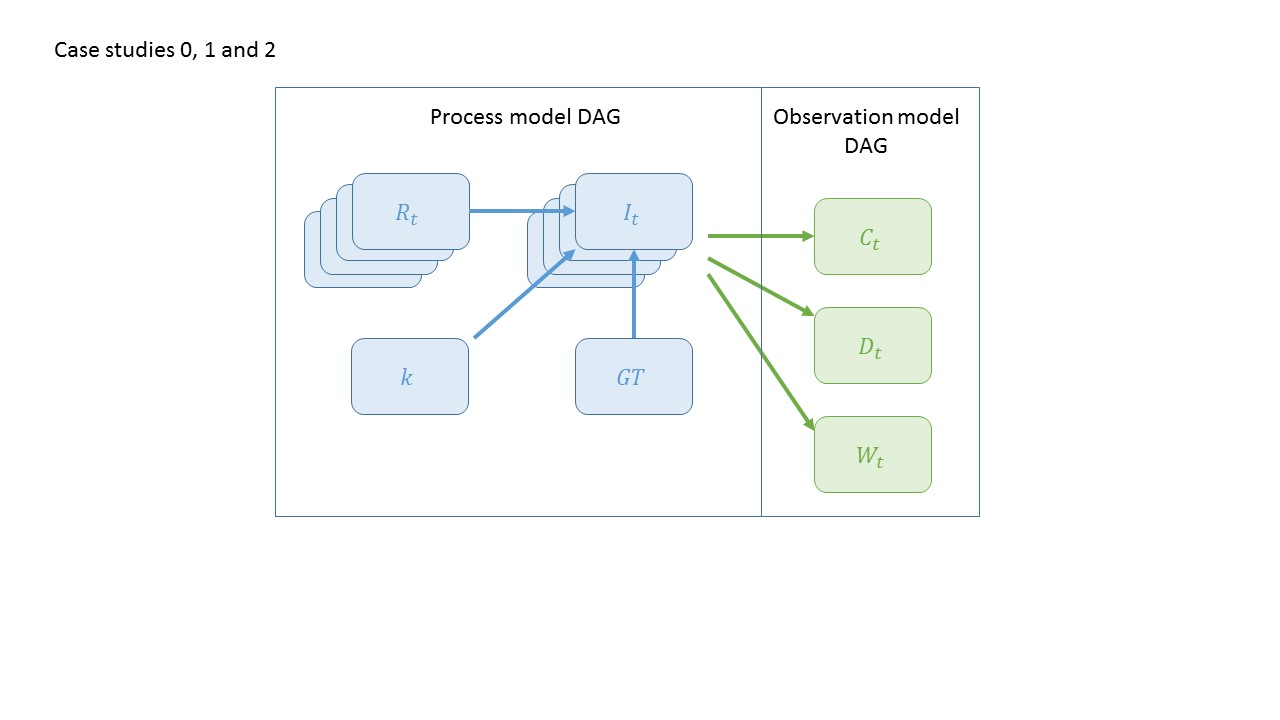
\includegraphics[width=0.75\textwidth]{figures/case_study_0_1_2.jpg}\\
(b)\\
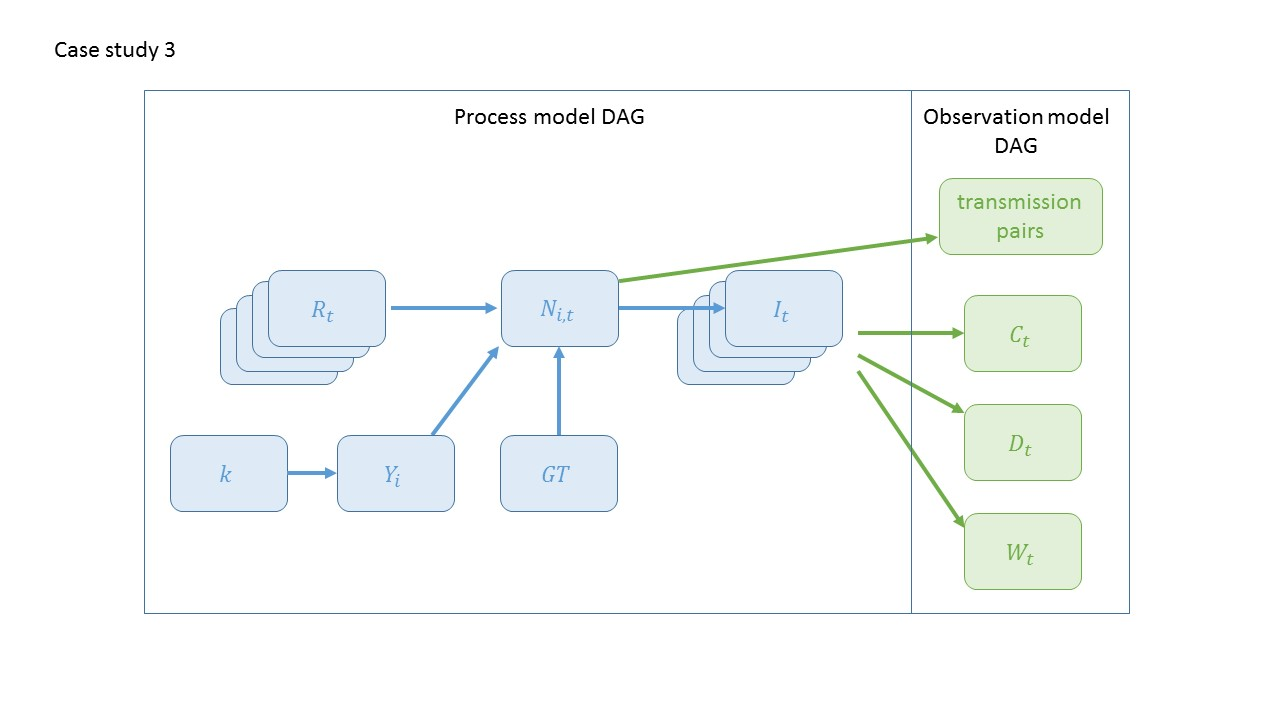
\includegraphics[width=0.75\textwidth]{figures/case_study_3.jpg}
\label{fig:CS3_DAG}
\caption{[Mike's attempt at DAGs for the case studies (can be made prettier later on).] Latent states in blue, observed states in green. (a) Case studies 0--2. Process model P1 is a special case where $I_t$ is a deterministic funcvtion of $R_t$ and $I_{1:t-1}$; P2 is a special case in the limit $k\to\infty$; P3 allowing the dispersion parameter $k$ to take any given value. The different observation models described in case study 0 (with or without underreporting, reporting delay, and observation noise) would affect how the expected value of the observed state $C_t$ relates to the latent states $I_{1:t}$, and the variance of the observed state $C_t$. Case studies 1 and 2 add additional observed states for deaths ($D_t$) and wasterwater observations ($W_t$) respectively. (b) Case study 3 requires more states to be inlcuded in the DAG to take account of individual heterogeneity and the impact it has on obsetved data on transmission pairs. The variable $N_{it}$ representing the number of secondary infections caused by individual $i$ on day $t$ encodes the full transmission tree. The expected value of $N_{it}$ is determined by the instantaneous reproduction number $R_t$, the relative transmission rates $Y_i$ of previously infected individuals, and their current infectiousness determined by the generation time distribution (GT). The variance in the distrubiton of $Y_i$ is determined by the dispersion parameter $k$.  }
\end{figure}






\section{Discussion}

\subsection{Summary}

We have presented a framework for integrating multiple data sources in infectious disease modelling that emphasises practical implementation through a structured, iterative workflow.
Our approach combines systematic model development using directed acyclic graphs with modular integration strategies that prioritise parsimony, interpretability, and explicit assessment of data source conflict.
The framework progresses from clear research question definition through process and observation DAG development to informed choices about integration methods, supported by expert survey evidence on data source characteristics and worked case studies demonstrating progressive complexity.
Key contributions include the structured workflow that makes modelling assumptions transparent, the expert consensus on data source trade-offs that guides selection decisions, and practical guidance that bridges the gap between methodological advances and real-world implementation challenges.
Our modular approach incentives building complexity incrementally, allowing practitioners to assess the value of additional data sources systematically whilst maintaining computational tractability and model interpretability.

\subsection{Strengths and Limitations}
% TODO: Strengths: Modular framework, practical focus rooted in SARS-CoV-2 experience across multiple countries, worked examples
% TODO: Strengths: Integration of diverse methodological approaches
% TODO: Strengths: Expert survey and empirical evidence base
% TODO: Limitations: Model selection and validation challenges
% TODO: Limitations: Dependence on data quality and availability
% TODO: Limitations: Computational considerations and scalability
% TODO: Limitations: perhaps we don't actually provide the code for the CSs. 
% I suggest starting with limitations and then having strenghts so it doesn't sound like we are shooting ourselves in the foot. 

\subsection{Comparison with Existing Literature}
% TODO: Position relative to pipeline vs joint modelling literature
% TODO: Relationship to evidence synthesis and meta-analysis methods
% TODO: Comparison with ensemble forecasting approaches
% TODO: Distinguish from existing reviews and methodological papers
% TODO: Compare with other multi-source integration frameworks

\subsection{Outstanding Challenges and Future Directions}
% TODO: Real-time implementation constraints and solutions
% TODO: Computational scalability for large-scale integration
% TODO: Methodological gaps in current approaches
% TODO: Emerging data sources and integration needs / opportunities
% TODO: Community standards and best practices
% TODO: Research priorities and next steps



\section{Conclusions}

Integrating multiple data sources offers substantial benefits for infectious disease modelling, but requires careful consideration of trade-offs between information gain, computational complexity, and interpretability.
Our framework provides infectious disease modellers with practical tools for navigating these choices through structured workflows, expert consensus on data characteristics, and demonstrated case studies that progress from single-source baselines to complex multi-stream integration.
The modular approach we advocate offers a pragmatic path forward that balances methodological rigor with practical considerations.
By making modelling assumptions explicit through DAG-based development and providing clear guidance on integration method selection, this framework enables more transparent, reproducible, and effective multi-source modelling.
We recommend that the infectious disease modelling community adopt these structured approaches and work towards establishing community standards for data integration that prioritise both methodological best practices and practical implementation needs.

\section{Acknowledgements}

All <placeholder> workshop participants for useful discussion and feedback. Poppy the dog for making sure to ask the important questions.

\bibliographystyle{plainnat}
\bibliography{references}


\end{document}
 